\documentclass[11pt,oneside,openany]{book}
\usepackage{notes}
% Macros specific to the unique games notes.
\newcommand{\val}{\operatorname{val}}
\newcommand{\OPT}{\operatorname{OPT}}
\newcommand{\cV}{\mathcal{V}}
\newcommand{\cW}{\mathcal{W}}
\newcommand{\GapUG}{\mathrm{GapUG}}


\title{Lecture Notes on the Unique Games Theorem}
\author{Abhijeet Mulgund}
\date{Version of October 29, 2026}

\begin{document}
\frontmatter
{\hypersetup{pageanchor=false}\maketitle}
\chapter*{Preface}

Written for readers new to hardness of approximation, these notes accompany a reading group on OpenAI's proof of the Unique Games Conjecture \cite{OAI}. They answer the question of Chapter~\ref{ch:ug}: how well can the value of a unique game be approximated in polynomial time? OpenAI's answer is Theorem~\ref{thm:ugt}.

\paragraph{Prerequisites.} Linear algebra over $\F_2$, Fourier analysis on finite abelian groups, and NP-hardness.

\paragraph{Route.} Part~I (Chapters~\ref{ch:outer}--\ref{ch:twotwo}) proves the 2-to-2 Games Theorem (Theorem~\ref{thm:2to2}) as a warm-up, with OpenAI's construction. Part~II (Chapters~\ref{ch:openai} and~\ref{ch:games}) changes that proof to obtain Theorem~\ref{thm:ugt}. Part~III, whose chapters will be added as the group reaches them, will prove the results that Part~II quotes from OpenAI's preprint.

\paragraph{Coverage.} Elementary facts are proved. H\aa stad's theorem, parallel repetition, an inverse theorem for the equality test (Theorem~\ref{thm:inverse}), Hoeffding's inequality, and several lemmas of OpenAI's preprint are quoted where they are used. A result marked ``after'' a source is proved here along the lines of that source.

\paragraph{Sources and status.} Definitions follow Khot's survey \cite{Khot10}, and notation follows OpenAI's preprint. OpenAI's proof is an unrefereed preprint (September 23, 2026) whose repository contains a Lean formalization. We know of no source for Part~I's assembly of the 2-to-2 proof in OpenAI's framework, so this assembly is new to these notes and has not been refereed. The notes were prepared with AI assistance (Claude).

\paragraph{Using the notes.} Each chapter ends with questions, and Appendix~\ref{app:answers} answers the questions. Later chapters do not depend on the questions. Appendix~\ref{app:notation} lists the notation. In the figures, blue marks what Part~II adds or replaces. The group's first session covered Chapters~\ref{ch:ug}--\ref{ch:twotwo}, and the second covers Chapters~\ref{ch:openai} and~\ref{ch:games}.

\tableofcontents

\mainmatter
\chapter{Unique games and the conjecture}\label{ch:ug}

The Unique Games Conjecture concerns how well the value of a unique game can be approximated in polynomial time.

\begin{definition}[Unique game]\label{def:ug}
A \emph{unique game} $G$ consists of a finite directed graph $(V,E)$ whose edges join distinct vertices (parallel edges allowed), a probability distribution $p$ on $E$ (the \emph{weights}; uniform unless stated), a finite alphabet $K$, and a permutation $\pi_e$ of $K$ for each edge $e=(v,w)$. A \emph{labeling} $\lambda:V\to K$ assigns each vertex $v$ a \emph{label} $\lambda(v)$, and
\[
\val_\lambda(G)=\Prob_{e=(v,w)\sim p}\bigl[\pi_e(\lambda(v))=\lambda(w)\bigr],\qquad \val(G)=\max_\lambda\val_\lambda(G).
\]
Here $\val_\lambda(G)$ is the probability that $\lambda$ satisfies a random edge, and $\val(G)$ is its maximum over labelings.
In a \emph{translation game}, $K=\F_2^N$ and $\pi_e(y)=y+b_e$ with $b_e\in K$ (Figure~\ref{fig:ugexample}).
\end{definition}

\begin{figure}[ht]
\centering
\begin{tikzpicture}[font=\small,
  v/.style={circle,draw,minimum size=6.5mm,inner sep=0pt},
  lab/.style={draw,rounded corners=1pt,inner sep=1.5pt,font=\footnotesize},
  off/.style={font=\footnotesize}]
\node[v] (u1) at (0,1.8) {$v_1$};
\node[v] (v1) at (4,1.8) {$v_2$};
\node[v] (u2) at (4,0) {$v_3$};
\node[v] (v2) at (0,0) {$v_4$};
\node[lab,left=2mm of u1] {$00$};
\node[lab,right=2mm of v1] {$01$};
\node[lab,right=2mm of u2] {$10$};
\node[lab,left=2mm of v2] {$10$};
\draw (u1) -- node[off,above] {$+01$} (v1);
\draw (v1) -- node[off,right] {$+11$} (u2);
\draw[dashed,thick] (u2) -- node[off,below] {$+01$} (v2);
\draw (v2) -- node[off,left] {$+10$} (u1);
\end{tikzpicture}
\caption{A translation game over $\F_2^2$ on a 4-cycle. Edge labels are the offsets $b_e$, and boxes show a labeling. Three edges are satisfied and the dashed one is not ($10+01\ne10$). The offsets sum to $01\ne00$ around the cycle, so a labeling satisfying all four edges would give $\lambda(v_1)=\lambda(v_1)+01$. Hence every labeling fails at least one of the four equally weighted edges, so $\val(G)\le3/4$, and the labeling shown attains $3/4$.}\label{fig:ugexample}
\end{figure}

For example, Max-Cut is the translation game over $\F_2$ with every $b_e=1$: a labeling is a cut, and an edge is satisfied when it crosses the cut.

\phantomsection\label{nt:gap}Hardness of approximating $\val(G)$ is stated through a decision problem. For $0<s<c\le1$, $\GapUG_K(c,s)$ is the problem of deciding, for a unique game over $K$ with $\val(G)\ge c$ or $\val(G)\le s$, which holds. Here $c$ is the \emph{completeness} and $s$ the \emph{soundness}. A polynomial-time algorithm that estimates $\val(G)$ with additive error less than $(c-s)/2$ would decide $\GapUG_K(c,s)$. So NP-hardness of $\GapUG_K(c,s)$ rules out such an algorithm unless $\mathrm{P}=\mathrm{NP}$. Khot conjectured that the gap can be almost as large as possible.

\begin{conjecture}[{Unique Games Conjecture, Khot 2002 \cite{Khot02}; see \cite[Conjecture~2.5]{Khot10}}]\label{conj:ugc}
For all $\varepsilon,\delta\in(0,1/2)$ there is a finite $K$ such that $\GapUG_K(1-\varepsilon,\delta)$ is NP-hard.
\end{conjecture}

Two facts show that the gap cannot be larger: the conjecture needs $\varepsilon>0$, and $K$ must grow as $\delta$ shrinks. First, whether $\val(G)=1$ is decidable in polynomial time: discard edges of probability zero, and in each connected component try every label at one vertex, propagate it along a spanning tree, and check every edge. So $\GapUG_K(1,s)$ is not NP-hard unless $\mathrm{P}=\mathrm{NP}$. Second, if $\lambda$ is a uniformly random labeling, then $\Prob_\lambda[\pi_e(\lambda(v))=\lambda(w)]=1/|K|$ for each edge $e$, so $\E_\lambda\val_\lambda(G)=1/|K|$ and some labeling has $\val_\lambda(G)\ge1/|K|$. So soundness $\delta$ requires $|K|\ge1/\delta$.

OpenAI proved the conjecture in the following form.

\begin{theorem}[{\cite[Theorem~1.1]{OAI}}]\label{thm:ugt}
For all $\varepsilon,\delta\in(0,1/2)$ there are $N\ge1$ and a polynomial-time reduction from 3SAT to unweighted (uniform $p$) translation games over $\F_2^N$ on simple bipartite graphs, with $\val\ge1-\varepsilon$ on satisfiable formulas and $\val\le\delta$ on unsatisfiable ones.
\end{theorem}

Chapter~\ref{ch:games} assembles its proof. Combined with earlier reductions that assume the conjecture, Theorem~\ref{thm:ugt} makes it NP-hard to approximate Max-Cut within any fixed ratio in $(\alpha_{\mathrm{GW}},1)$, where $\alpha_{\mathrm{GW}}\approx0.878$ is the Goemans--Williamson constant, and Vertex Cover within any fixed factor in $(1,2)$ \cite[Section~8.1]{OAI}.

Before OpenAI's proof, the strongest result of this form had completeness $1/2$ \cite[Theorem~2.20]{Khot19}. It comes from games with a weaker kind of constraint. A \emph{2-to-2 constraint} on $K\times K$ is a relation $\mathcal R=\bigcup_{j=1}^{|K|/2}B_j\times B'_j$, where $B_1,\dots,B_{|K|/2}$ and $B'_1,\dots,B'_{|K|/2}$ are two partitions of $K$ into sets of size $2$. If $y\in B_j$, then $(y,y')\in\mathcal R$ exactly for the two elements $y'$ of $B'_j$. Likewise, each $y'\in B'_j$ is related exactly to the two elements of $B_j$. Hence the name (Figure~\ref{fig:twotwodef}). A \emph{2-to-2 game} is defined like a unique game (Definition~\ref{def:ug}) with 2-to-2 constraints in place of permutations.

\begin{figure}[ht]
\centering
\begin{tikzpicture}[font=\small,
  lb/.style={inner sep=2pt,minimum width=1.3cm}]
\node[lb] (l1) at (0,3) {$y_0$};
\node[lb] (l2) at (0,2.2) {$y_1$};
\node[lb] (l3) at (0,1) {$\tilde y_0$};
\node[lb] (l4) at (0,0.2) {$\tilde y_1$};
\node[lb] (r1) at (4,3) {$y'_0$};
\node[lb] (r2) at (4,2.2) {$y'_1$};
\node[lb] (r3) at (4,1) {$\tilde y'_0$};
\node[lb] (r4) at (4,0.2) {$\tilde y'_1$};
\node[draw,rounded corners=3pt,fit=(l1)(l2),inner sep=1pt,label=left:{$B_j$}] {};
\node[draw,rounded corners=3pt,fit=(l3)(l4),inner sep=1pt,label=left:{$B_{\tilde j}$}] {};
\node[draw,rounded corners=3pt,fit=(r1)(r2),inner sep=1pt,label=right:{$B'_j$}] {};
\node[draw,rounded corners=3pt,fit=(r3)(r4),inner sep=1pt,label=right:{$B'_{\tilde j}$}] {};
\node[above=0.45cm] at (l1) {$y\in K$};
\node[above=0.45cm] at (r1) {$y'\in K$};
\foreach \i in {1,2,3,4} { \draw[thick] (l\i.east) -- (r\i.west); }
\draw[dashed] (l1.east) -- (r2.west);
\draw[dashed] (l2.east) -- (r1.west);
\draw[dashed] (l3.east) -- (r4.west);
\draw[dashed] (l4.east) -- (r3.west);
\node at (0,-0.55) {$\vdots$};
\node at (4,-0.55) {$\vdots$};
\draw[thick] (6.2,2.2) -- (7.0,2.2) node[right] {$\sigma_0(y_i)=y'_i$};
\draw[dashed] (6.2,1.2) -- (7.0,1.2) node[right] {$\sigma_1(y_i)=y'_{i+1}$};
\end{tikzpicture}
\caption{A 2-to-2 constraint $\mathcal R$: all four pairs between $B_j$ and $B'_j$ are related. Two of the $|K|/2$ pairs of blocks are shown. The solid and dashed edges are the graphs of the two permutations $\sigma_0$ and $\sigma_1$ of Lemma~\ref{lem:split}, with indices in $\F_2$.}\label{fig:twotwodef}
\end{figure}

\begin{theorem}[{2-to-2 Games Theorem: Khot--Minzer--Safra 2018 \cite{KMS23}; see \cite[Theorem~2.19]{Khot19}}]\label{thm:2to2}
For every $\varepsilon\in(0,1/2)$ there is a finite alphabet for which distinguishing 2-to-2 games with $\val\ge1-\varepsilon$ from those with $\val\le\varepsilon$ is NP-hard.
\end{theorem}

A 2-to-2 constraint is the union of the graphs of two permutations, and imposing one of them at random halves every value.

\begin{lemma}\label{lem:split}
A 2-to-2 constraint $\mathcal R=\bigcup_jB_j\times B'_j$ is $\mathrm{graph}(\sigma_0)\sqcup\mathrm{graph}(\sigma_1)$ for two permutations $\sigma_0,\sigma_1$ of $K$. So if $G$ is a 2-to-2 game and $G'$ samples $e\sim p$ as $G$ does and then imposes $\sigma_0$ or $\sigma_1$ with probability $1/2$ each, then $\val_\lambda(G')=\val_\lambda(G)/2$ for every labeling $\lambda$.
\end{lemma}

\begin{proof}
Write each pair of blocks as $B_j=\{y_0,y_1\}$ and $B'_j=\{y'_0,y'_1\}$, with indices in $\F_2$, and define $\sigma_c(y_i)=y'_{i+c}$ for $c\in\F_2$. Since $\{B_j\}$ and $\{B'_j\}$ partition $K$, $\sigma_0$ and $\sigma_1$ are permutations of $K$. For $y\in B_j$, the two elements of $B'_j$ are $\sigma_0(y)\ne\sigma_1(y)$. So if $(y,y')\in\mathcal R$, then $y'$ equals exactly one of them, and if $(y,y')\notin\mathcal R$, it equals neither. Hence, given $e$, a labeling that satisfies $e$ satisfies the chosen permutation with probability exactly $1/2$, and a labeling that fails $e$ satisfies neither permutation. So $\val_\lambda(G')=\val_\lambda(G)/2$.
\end{proof}

So splitting the constraints of the games in Theorem~\ref{thm:2to2} gives unique games with completeness $(1-\varepsilon)/2$.

\begin{corollary}[{\cite[Section~2.8]{Khot19}}]\label{cor:half}
For all $\varepsilon\in(0,1)$ and $\delta\in(0,(1-\varepsilon)/2)$ there is a finite $K$ such that $\GapUG_K\bigl((1-\varepsilon)/2,\delta\bigr)$ is NP-hard.
\end{corollary}

\begin{proof}
Apply Theorem~\ref{thm:2to2} with $\varepsilon_0=\min\{\varepsilon,2\delta,1/4\}$ in place of $\varepsilon$, and split every constraint as in Lemma~\ref{lem:split}. Splitting halves every value. So instances with $\val\ge1-\varepsilon_0$ become unique games with $\val\ge(1-\varepsilon_0)/2\ge(1-\varepsilon)/2$, and instances with $\val\le\varepsilon_0$ become unique games with $\val\le\varepsilon_0/2\le\delta$.
\end{proof}

How are the two theorems related? Corollary~\ref{cor:half} stops at completeness $(1-\varepsilon)/2$ because splitting halves every value (Lemma~\ref{lem:split}). Part~I proves Theorem~\ref{thm:2to2} with the construction that OpenAI uses for Theorem~\ref{thm:ugt}, but with 2-to-2 constraints where OpenAI's construction has permutations. Part~II replaces them by permutations. This changes one step of the soundness proof, and the new step yields soundness only $0.99$, which Chapter~\ref{ch:games} shows is enough.

\chapternotes
Unique games had been studied in the context of parallel repetition before Khot posed the problem of approximating their value \cite[Section~2.4]{Khot10}. Khot's survey \cite{Khot10} is the source of the definitions used here and describes the consequences of the conjecture known in 2010. The proof of Theorem~\ref{thm:2to2} is spread over four papers of Khot, Minzer, and Safra and of Dinur, Khot, Kindler, Minzer, and Safra \cite{KMS17,DKKMS,DKKMS21,KMS23}. Khot's exposition \cite{Khot19} lists them in its abstract and gives an overview of the whole proof.

\chapterquestions
\begin{question}\label{q:oddcycle}
Let $G$ be Max-Cut on a cycle $v_1,\dots,v_L$ of odd length $L$: the translation game over $\F_2$ with edges $(v_i,v_{i+1})$ for $i=1,\dots,L$, where $v_{L+1}=v_1$, every $b_e=1$, and uniform weights. Compute $\val(G)$.
\end{question}

\begin{question}\label{q:propagation}
Where does the algorithm that decides whether $\val(G)=1$ (after Conjecture~\ref{conj:ugc}) use that each $\pi_e$ is a permutation? What does the same procedure do on a 2-to-2 game?
\end{question}

\part{The 2-to-2 Games Theorem by OpenAI's method}

Part~I proves Theorem~\ref{thm:2to2}. Part~I's reduction from 3SAT has two parts: a projection game built from parity equations (Chapter~\ref{ch:outer}), and new vertices with constraints between them that turn this game into a 2-to-2 game (Chapter~\ref{ch:inner}). Soundness rests on an inverse theorem for the equality test (Chapter~\ref{ch:soundness}) and on a decoding argument (Chapter~\ref{ch:twotwo}).

The construction is OpenAI's \cite[Section~4]{OAI}, with 2-to-2 constraints where OpenAI's reduction has permutations. The 2-to-2 proof in the literature works instead with subspaces and a bipartite 2-to-1 game \cite[Sections~4--5]{DKKMS}, and it states the 2-to-2 form without a separate proof \cite[Theorem~1.11]{DKKMS}. So Part~I follows the steps of Dinur, Khot, Kindler, Minzer, and Safra inside OpenAI's framework.

\chapter{A projection game from parity equations}\label{ch:outer}

How can a reduction from 3SAT produce games in which each constraint involves only two vertices? OpenAI's construction, used in both parts of these notes, first produces a \emph{projection game} from H\aa stad's parity equations. Its constraints are maps rather than permutations. The construction of Chapter~\ref{ch:inner} relies on exactly this: when the constraint of an edge is a map, the label at one endpoint determines the label that the other endpoint must have.

\begin{definition}[Projection game]\label{def:projection}
A \emph{projection game} $G$ consists of a finite bipartite graph $(V,W,E)$ with a probability distribution $p$ on $E$, a finite alphabet $\Sigma_v$ for each $v\in V$ and $\Sigma_w$ for each $w\in W$, and a map $\pi_e:\Sigma_v\to\Sigma_w$ for each edge $e=(v,w)$. A labeling assigns a label $\lambda(v)\in\Sigma_v$ to each $v\in V$ and $\lambda(w)\in\Sigma_w$ to each $w\in W$, and $\val(G)=\max_\lambda\Prob_{e=(v,w)\sim p}\bigl[\pi_e(\lambda(v))=\lambda(w)\bigr]$.
\end{definition}

A bipartite unique game is the special case in which all alphabets equal one $K$ and every $\pi_e$ is a bijection. Projection games are often described as interactions of a verifier with two provers, and these notes use that language only for the advice experiment of Chapters~\ref{ch:twotwo} and~\ref{ch:openai}, where what each prover receives matters. A \emph{verifier} samples $e=(v,w)\sim p$, sends $v$ to a first \emph{prover} and $w$ to a second, and accepts if the labels $\lambda(v),\lambda(w)$ that the provers return satisfy $\pi_e(\lambda(v))=\lambda(w)$. A \emph{strategy} for the provers is a labeling, and the verifier accepts with probability $\val_\lambda(G)$.

The starting point is H\aa stad's theorem: approximating systems of parity equations is NP-hard.

\begin{theorem}[{H\aa stad 2001 \cite[Theorem~5.4 and its proof]{Hastad01}; see also \cite[Theorem~22.16 and Section~22.4.1]{AB09}}]\label{thm:hastad}
For every $\xi\in(0,1/4)$, the following problem is NP-hard. A system $\Theta$ consists of equations $x+x'+x''=b$ over $\F_2$ in variables from a set $X$, together with a probability distribution $p$ on the equations. Let $\OPT(\Theta)=\max_{\mathbf x\in\F_2^X}\Prob_{\theta\sim p}[\mathbf x\text{ satisfies }\theta]$. Given $\Theta$ with $\OPT(\Theta)\ge1-\xi$ or $\OPT(\Theta)\le1/2+\xi$, decide which holds.
\end{theorem}

Both constants in Theorem~\ref{thm:hastad} are optimal, for the two reasons met in Chapter~\ref{ch:ug}. With $\xi=0$ the problem is in P (Gaussian elimination), so NP-hardness requires completeness below $1$ unless $\mathrm{P}=\mathrm{NP}$. And $\OPT(\Theta)\ge1/2$ for every system: some variable occurs an odd number of times in each equation, so a uniformly random assignment $\mathbf x$ satisfies each equation with probability exactly $1/2$, and $\E_{\mathbf x}\Prob_{\theta\sim p}[\mathbf x\text{ satisfies }\theta]=1/2$. So when $\OPT(\Theta)\le1/2+\xi$, every assignment $\mathbf x$ has $\Prob_{\theta\sim p}[\mathbf x\text{ satisfies }\theta]$ at most $\xi$ above its average $1/2$ over uniformly random $\mathbf x$.

To make a projection game, pair each equation with each of its variables. This construction requires the three variables of every equation to be distinct. For $\xi<1/100$, OpenAI's Lemma~4.2 replaces each system $\Theta$ of Theorem~\ref{thm:hastad} by a system $\Theta'$ with three distinct variables in each equation, such that $\OPT(\Theta')\ge1-\xi$ if $\OPT(\Theta)\ge1-\xi$ (the \emph{YES case}) and $\OPT(\Theta')\le4/5$ if $\OPT(\Theta)\le1/2+\xi$ (the \emph{NO case}) \cite[Lemma~4.2]{OAI}. From now on, $\Theta$ denotes the new system.

\begin{definition}[Equation-versus-variable game]\label{def:evv}
For a system $\Theta$ on variables $X$, with distribution $p$ and three distinct variables in each equation, $G_\Theta$ is the projection game with $V=\Theta$, $W=X$, and an edge $(\theta,x)$ for each equation $\theta$ and each of its three variables $x$. Its random edge is $(\theta,x)$ with $\theta\sim p$ and $x$ uniform among the variables of $\theta$. The alphabet $\Sigma_\theta$ is the set of four satisfying assignments $\phi$ of the variables of $\theta$, the alphabet of a variable is $\Sigma_x=\F_2$, and $\pi_{(\theta,x)}(\phi)=\phi(x)$ (Figure~\ref{fig:evv}).
\end{definition}

\begin{figure}[ht]
\centering
\begin{tikzpicture}[font=\small,a/.style={draw,rounded corners=1pt,inner sep=2pt,minimum width=9mm}]
\node at (0,2.25) {$\theta:\ x_1+x_2+x_3=1$};
\node[a] (a1) at (0,1.5) {$100$};
\node[a] (a2) at (0,0.9) {$010$};
\node[a] (a3) at (0,0.3) {$001$};
\node[a] (a4) at (0,-0.3) {$111$};
\node at (4,2.25) {variable $x_2$};
\node[a] (b0) at (4,1.2) {$0$};
\node[a] (b1) at (4,0.0) {$1$};
\foreach \s/\t in {a1/b0,a3/b0,a2/b1,a4/b1} \draw[-{Stealth[length=1.6mm]}] (\s.east) -- (\t.west);
\node at (2,1.85) {$\pi_e$};
\end{tikzpicture}
\caption{One edge $e=(\theta,x_2)$ of $G_\Theta$. Each bit has two preimages under $\pi_e$, so $\pi_e$ is 2-to-1.}\label{fig:evv}
\end{figure}

The value of $G_\Theta$ is at least $\OPT(\Theta)$: label the variables by a best assignment, and each equation it satisfies by its restriction. In the YES case, $\val(G_\Theta)\ge1-\xi$. Lemma~\ref{lem:evv} bounds $\val(G_\Theta)$ from above.

\begin{lemma}\label{lem:evv}
$\val(G_\Theta)\le1-\bigl(1-\OPT(\Theta)\bigr)/3$.
\end{lemma}

\begin{proof}
Fix a labeling $\lambda$. Its labels $\lambda(x)\in\F_2$ of the variables form an assignment of $\Theta$. Recall from Definition~\ref{def:evv} that the random edge is $(\theta,x)$, with $\theta\sim p$ and $x$ uniform among the three variables of $\theta$, and that it fails exactly when $\phi(x)\ne\lambda(x)$, where $\phi=\lambda(\theta)$.

Fix an equation $\theta$ that the assignment violates. Its label $\phi$ satisfies $\theta$, so some variable $x^*$ of $\theta$ has $\phi(x^*)\ne\lambda(x^*)$. Given $\theta$, the edge therefore fails with conditional probability at least $\Prob[x=x^*]=1/3$.

The assignment violates $\theta\sim p$ with probability at least $1-\OPT(\Theta)$. Hence the random edge fails with probability at least $\tfrac13\bigl(1-\OPT(\Theta)\bigr)$, which is the claim.
\end{proof}

With $\OPT(\Theta)\le4/5$, Lemma~\ref{lem:evv} gives $\val(G_\Theta)\le14/15$.

A value of at most $14/15$ is far from small. Repetition draws $n$ independent random edges at once and requires one labeling of the $n$-tuples to satisfy all of them.

\begin{definition}[Repetition]\label{def:rep}
For $n\ge1$, the \emph{$n$-fold repetition} $G^{\otimes n}$ is the projection game on $(V^n,W^n)$ in which a vertex $(v_1,\dots,v_n)$ has alphabet $\Sigma_{v_1}\times\cdots\times\Sigma_{v_n}$, and likewise on $W^n$. Its random edge $\mathbf e=(e_1,\dots,e_n)$ has independent entries $e_i\sim p$, and its projection is $\pi_{\mathbf e}=\pi_{e_1}\times\cdots\times\pi_{e_n}$.
\end{definition}

A labeling of $G^{\otimes n}$ need not act entry by entry, so $\val(G^{\otimes n})$ can exceed $\val(G)^n$. The value still decays exponentially, at a rate that does not depend on the alphabet.

\begin{theorem}[{Rao 2011 \cite{Rao11}; Dinur--Steurer 2014 \cite[Corollary~1.2]{DS14}}]\label{thm:rep}
Let $G$ be a projection game, $n\ge1$, and $\Delta\in(0,1)$. If $\val(G)\le1-\Delta$, then $\val(G^{\otimes n})\le(1-\Delta^2/16)^n$, whatever the alphabets.
\end{theorem}

Theorem~\ref{thm:rep} makes the value of a repetition of $G_\Theta$ small in the NO case. The soundness proof of Chapter~\ref{ch:twotwo} also uses that the two endpoints of a random edge differ in few entries, fewer than about $\sqrt k$ (Lemma~\ref{lem:tv}). In $G_\Theta^{\otimes k}$ they differ in every entry, since one endpoint is a tuple of equations and the other a tuple of variables. The smooth game replaces each equation only with a small probability $\beta$.

\begin{definition}[Smooth $k$-fold game]\label{def:smooth}
For $k\ge1$ and $\beta\in(0,1)$, the \emph{smooth $k$-fold game} is the projection game whose random edge $(U,O)$ is drawn as follows. Its first endpoint is $U=(\theta_1,\dots,\theta_k)$ with independent $\theta_i\sim p$. Independently for each $i$, let $o_i=\theta_i$ with probability $1-\beta$, and otherwise let $o_i$ be a uniformly random variable of $\theta_i$. The second endpoint is $O=(o_1,\dots,o_k)$ (Figure~\ref{fig:smooth}). The alphabet $\Sigma_U$ is the product of the alphabets of $\theta_1,\dots,\theta_k$, and $\Sigma_O$ the product of the alphabets of $o_1,\dots,o_k$, with separate factors for repeated equations or variables. The projection maps a label $(\phi_1,\dots,\phi_k)$ of $U$ to the label of $O$ whose $i$th entry is $\phi_i$ if $o_i=\theta_i$ and $\phi_i(o_i)$ if $o_i$ is a variable.
\end{definition}

In the YES case, a best assignment satisfies all $k$ equations of $U$ with probability at least $1-k\xi$, by a union bound. If $\beta=0$, then $O=U$ and the smooth game has value $1$, so $\beta$ must be positive. Chapter~\ref{ch:twotwo} needs both $\beta k\to\infty$, so that the number of replaced entries grows and Theorem~\ref{thm:rep} applies to them (Lemma~\ref{lem:clean}), and $k\beta^2\to0$, for the comparison of laws in Lemma~\ref{lem:tv}. OpenAI takes $\beta=k^{-2/3}$, so $\beta k=k^{1/3}\to\infty$ and $k\beta^2=k^{-1/3}\to0$.

\begin{figure}[ht]
\centering
\begin{tikzpicture}[font=\small,
  eq/.style={draw,minimum width=0.95cm,minimum height=0.6cm},
  var/.style={draw,circle,minimum size=0.6cm,inner sep=0pt}]
\node at (-0.9,1.2) {$U$};
\node at (-0.9,0) {$O$};
\foreach \i in {1,...,8} {
  \node[eq] (u\i) at ({1.15*(\i-1)},1.2) {$\theta_{\i}$};
}
\foreach \i in {1,2,4,5,7,8} {
  \node[eq] (o\i) at ({1.15*(\i-1)},0) {$\theta_{\i}$};
  \draw[-{Stealth[length=1.6mm]}] (u\i) -- (o\i);
}
\foreach \i in {3,6} {
  \node[var] (o\i) at ({1.15*(\i-1)},0) {$x$};
  \draw[-{Stealth[length=1.6mm]},dashed] (u\i) -- (o\i);
}
\node[right,font=\footnotesize] at (8.6,1.2) {first endpoint};
\node[right,font=\footnotesize] at (8.6,0) {second endpoint};
\end{tikzpicture}
\caption{A random edge $(U,O)$ of the smooth game ($k=8$). Each equation is replaced with probability $\beta$ by one of its variables ($x$), chosen uniformly.}\label{fig:smooth}
\end{figure}

\paragraph{Labels as vectors.}\phantomsection\label{nt:labels} Chapter~\ref{ch:inner} encodes a label by evaluating linear maps on it, so the labels of the smooth game must be vectors and its projections linear maps. Each vertex $Q$ of the smooth game is a $k$-tuple whose entries are equations or variables: every entry of $U$ is an equation, and an entry of $O$ is a variable wherever an equation was replaced. A label of $Q$ assigns each equation entry one of its four satisfying assignments and each variable entry a bit. A satisfying assignment $(\phi_1,\phi_2,\phi_3)$ of an equation with right side $b$ is determined by $(\phi_1,\phi_2)$, since $\phi_3=b+\phi_1+\phi_2$. So a label of $Q$ is a list of $d_Q$ bits, two for each equation entry and one for each variable entry. In these bits, restriction to $O$ is affine but in general not linear: a variable entry of $O$ may receive the value $\phi_3=b+\phi_1+\phi_2$, which has the constant term $b$. One extra coordinate removes the constant. Let $L_Q=\F_2^{1+d_Q}$, with coordinates indexed from $0$, and represent a label by the vector $z\in L_Q$ with $z_0=1$ followed by its $d_Q$ bits. The coordinate $z_0$ is the \emph{homogeneous coordinate}. Since $\phi_3=bz_0+\phi_1+\phi_2$ is linear in $z$, restriction extends to a linear map $\bar\pi:L_U\to L_O$ that keeps the homogeneous coordinate, $(\bar\pi z)_0=z_0$ \cite[Section~4.2]{OAI}. The labels of $Q$ are exactly the vectors $z\in L_Q$ with $z_0=1$. For a first endpoint $U$, $d_U=2k$, so $L_U=\F_2^m$ with $m=1+2k$.

\chapterquestions
\begin{question}\label{q:evvexact}
Show that Lemma~\ref{lem:evv} is an equality: $\val(G_\Theta)=1-\bigl(1-\OPT(\Theta)\bigr)/3$.
\end{question}

\begin{question}\label{q:pibar}
Let $k=1$ and $U=(\theta)$ with $\theta:\ x_1+x_2+x_3=b$, and give $L_U$ the coordinates $(z_0,\phi_1,\phi_2)$. Write the matrix of $\bar\pi$ when $O$ replaces $\theta$ by $x_3$, and when $O$ replaces $\theta$ by $x_1$. Which of the two restrictions is linear on the bits $(\phi_1,\phi_2)$ without the homogeneous coordinate?
\end{question}

\chapter{Clouds, tests, and the 2-to-2 game}\label{ch:inner}

The smooth game is a projection game, not a unique game. On an edge $(U,O)$, each replaced equation makes the projection 2-to-1 in its entry, as in Figure~\ref{fig:evv}, so the projection is many-to-one unless no equation was replaced. How can its labels be checked by constraints between single elements of a small alphabet $K$? OpenAI's construction replaces each first endpoint of the smooth game by a set of new vertices, called its cloud, whose labelings encode labels of the endpoint, and it puts constraints inside each cloud that encodings of labels satisfy. For Part~I, the answer is the 2-to-2 game $G_{2:2}$ of Definition~\ref{def:G22}, whose value is at least $1-k\xi-2^{-\ell}-2^{1-m}$ when $\OPT(\Theta)\ge1-\xi$.

\paragraph{Clouds and encodings.}\phantomsection\label{nt:clouds} Fix $\ell\ge1$. A \emph{table} on a vertex $Q$ of the smooth game is a linear map $P:L_Q\to\F_2^\ell$, and the \emph{encoding} of a label $z\in L_Q$ is the function $P\mapsto Pz$ on tables. On a first endpoint $U$, the tables are the matrices $M\in\Mat_{\ell,m}=\Hom(L_U,\F_2^\ell)$, and the encoding of $z$ is $f_z(M)=Mz$. Each table on a first endpoint $U$ gives a vertex of a new game, with labels in $K=\F_2^\ell$. Tables on different first endpoints can give the same vertex, as the next paragraph explains. The tables on $U$ form the \emph{cloud} of $U$, and the encoding $f_z$ of a label $z$ of $U$ is a labeling of this cloud (Figure~\ref{fig:layers}).

\paragraph{Shared vertices.}\phantomsection\label{nt:shared} Clouds are joined through the second endpoints. A table $P'$ on $O$ gives the table $P'\bar\pi=P'\circ\bar\pi$ on $U$, its \emph{pullback} along $\bar\pi$. For every $z\in L_U$, $(P'\bar\pi)z=P'(\bar\pi z)$: the encoding of $z$ at the pullback equals the encoding of the restriction $\bar\pi z$ at $P'$. In OpenAI's reduction, a table $P'$ on $O$ and its pullbacks to all first endpoints $U$ with an edge $(U,O)$ are a single vertex\footnote{OpenAI's vertices are $K$-orbits of \emph{keys}, where the key of a table is a reduced form of it that keeps, in each entry, only the coordinates on which the table depends \cite[Section~4.3]{OAI}. A table on $O$ and its pullbacks have the same key, and other tables can share a key too.}, shared by the clouds of these $U$. Suppose the clouds of $U_1$ and $U_2$ are labeled by the encodings of $z_{U_1}$ and $z_{U_2}$, and let $\bar\pi_1$ and $\bar\pi_2$ be the restrictions from $U_1$ and $U_2$ to $O$. The shared vertex $P'$ then receives the label $P'(\bar\pi_1z_{U_1})$ from one cloud and $P'(\bar\pi_2z_{U_2})$ from the other. These agree for every table $P'$ on $O$ exactly when $\bar\pi_1z_{U_1}=\bar\pi_2z_{U_2}$, that is, when $z_{U_1}$ and $z_{U_2}$ restrict to the same label of $O$. So encodings $f_{z_U}$ of labels $z_U$, one on each cloud, take the same value at all pullbacks of each table on a second endpoint exactly when the labels $z_U$ come from a labeling of the smooth game that satisfies every edge. Hence the names: the smooth game is the \emph{outer game}, which determines the vertices that clouds share, and the constraints inside the clouds form the \emph{inner test}.

\begin{figure}[ht]
\centering
\begin{tikzpicture}[font=\small,
  dot/.style={circle,fill,inner sep=1.3pt},
  qv/.style={draw,circle,inner sep=1pt,minimum size=7mm}]
\node[qv] (u1) at (0.2,2.7) {$U_1$};
\node[qv] (o) at (1.9,2.7) {$O$};
\node[qv] (u2) at (3.6,2.7) {$U_2$};
\draw[-{Stealth[length=2mm]}] (u1) -- (o);
\draw[-{Stealth[length=2mm]}] (u2) -- (o);
\node[right,align=left] at (5.9,2.7) {outer game:\\edges of the smooth game};
\draw (0.2,0) ellipse (1.85 and 0.95);
\draw (3.6,0) ellipse (1.85 and 0.95);
\node at (-0.6,1.2) {cloud of $U_1$};
\node at (4.4,1.2) {cloud of $U_2$};
\node[dot] (a1) at (-0.9,0.35) {};
\node[dot] (a2) at (-0.4,-0.45) {};
\node[dot] (a3) at (0.5,0.5) {};
\node[dot] (s1) at (1.9,0.3) {};
\node[dot] (s2) at (1.9,-0.3) {};
\node[dot] (b1) at (3.3,0.5) {};
\node[dot] (b2) at (3.8,-0.45) {};
\node[dot] (b3) at (4.6,0.3) {};
\draw (a1) -- (a2); \draw (a2) -- (s2); \draw (a3) -- (s1);
\draw (s1) -- (b1); \draw (s2) -- (b2); \draw (b2) -- (b3);
\node[font=\footnotesize,align=center] (sl) at (1.9,-1.55) {shared vertices: a table $P'$ on $O$\\and its pullbacks $P'\bar\pi$};
\draw[-{Stealth[length=1.6mm]}] (sl) -- (s2);
\node[right,align=left] at (5.9,0) {new game: tables are its vertices,\\and a table on $O$ and its\\pullbacks count as one vertex.\\Inner-test edges join\\tables of one cloud.};
\end{tikzpicture}
\caption{The two layers in OpenAI's reduction (schematic). The edges of the outer game (top) determine which vertices the clouds of $U_1$ and $U_2$ share (bottom).}\label{fig:layers}
\end{figure}

Each inner test in these notes compares the labels at two tables $M$ and $M+al^\top$ of one cloud, where $a$ and $l$ are random vectors, so the two tables differ by a matrix of rank at most one.

\begin{definition}[{2-to-2 test: Barak, Kothari, and Steurer 2018 \cite[Section~1.3, Test~2]{BKS18}; equality test: \cite[Section~1.4]{OAI}}]\label{def:shortcode}
The encoding $f_z(M)=Mz$ of $z\in\F_2^m$ is its \emph{degree-2 shortcode}. For $f:\Mat_{\ell,m}\to\F_2^\ell$ and independent uniform $M\in\Mat_{\ell,m}$, $a\in\F_2^\ell$, $l\in\F_2^m$, the \emph{2-to-2 test} accepts if $f(M+al^\top)-f(M)\in\{0,a\}$, and the \emph{equality test} accepts if $f(M+al^\top)=f(M)$.
\end{definition}

Encodings pass the two tests with different probabilities.

\begin{lemma}\label{lem:completeness}
For $z\ne0$, $f_z$ passes the 2-to-2 test with probability $1$ and the equality test with probability $(1+2^{-\ell})/2$.
\end{lemma}

\begin{proof}
By linearity, $f_z(M+al^\top)-f_z(M)=a(l^\top z)\in\{0,a\}$, so the 2-to-2 test always accepts. The equality test accepts exactly when $l^\top z=0$ or $a=0$. Since $z\ne0$, the bit $l^\top z$ is uniform and independent of $a$, so this event has probability $\tfrac12+\tfrac12\cdot2^{-\ell}$.
\end{proof}

So encodings pass the 2-to-2 test with probability $1$, but its constraint is not a permutation. The equality test imposes a permutation, but encodings pass it with probability only $(1+2^{-\ell})/2$. Part~I uses the 2-to-2 test and obtains 2-to-2 games. Part~II replaces it by a test whose constraints are permutations and which encodings pass with probability close to $1$. For $a\ne0$, the 2-to-2 test imposes a 2-to-2 constraint (Chapter~\ref{ch:ug}) on $\bigl(f(M),f(M+al^\top)\bigr)$, whose blocks $B_j=B'_j$ are the $|K|/2$ cosets $\{y,y+a\}$ of $\{0,a\}$ (Figure~\ref{fig:twotwo}). Splitting it by Lemma~\ref{lem:split} gives the identity $\sigma_0$, which is the constraint of the equality test, and the translation $\sigma_1(y)=y+a$. The encoding $f_z$ satisfies $\sigma_0$ exactly when $a(l^\top z)=0$, and $\sigma_1$ exactly when $a(l^\top z)=a$. Given $a\ne0$, each event has probability exactly $1/2$, so splitting halves the completeness, as in Corollary~\ref{cor:half}.

\begin{figure}[ht]
\centering
\begin{tikzpicture}[font=\small,
  lb/.style={inner sep=2pt,minimum width=1.3cm}]
\node[lb] (l1) at (0,3) {$y$};
\node[lb] (l2) at (0,2.2) {$y+a$};
\node[lb] (l3) at (0,1) {$\tilde y$};
\node[lb] (l4) at (0,0.2) {$\tilde y+a$};
\node[lb] (r1) at (4,3) {$y$};
\node[lb] (r2) at (4,2.2) {$y+a$};
\node[lb] (r3) at (4,1) {$\tilde y$};
\node[lb] (r4) at (4,0.2) {$\tilde y+a$};
\foreach \n in {l,r} {
  \node[draw,rounded corners=3pt,fit=(\n1)(\n2),inner sep=1pt] {};
  \node[draw,rounded corners=3pt,fit=(\n3)(\n4),inner sep=1pt] {};
}
\node[above=0.45cm] at (l1) {label at $M$};
\node[above=0.45cm] at (r1) {label at $M+al^\top$};
\foreach \i in {1,2,3,4} { \draw[thick] (l\i.east) -- (r\i.west); }
\draw[dashed] (l1.east) -- (r2.west);
\draw[dashed] (l2.east) -- (r1.west);
\draw[dashed] (l3.east) -- (r4.west);
\draw[dashed] (l4.east) -- (r3.west);
\node at (0,-0.55) {$\vdots$};
\node at (4,-0.55) {$\vdots$};
\draw[thick] (6.0,2.2) -- (6.8,2.2) node[right] {$\sigma_0=$ identity: the equality test};
\draw[dashed] (6.0,1.2) -- (6.8,1.2) node[right] {$\sigma_1=$ translation by $a$};
\end{tikzpicture}
\caption{For $a\ne0$, the constraint of the 2-to-2 test is the union of the graphs of two permutations (Lemma~\ref{lem:split}). Two of the $|K|/2$ blocks are shown. Indexing each block $\{y,y+a\}$ by $y_0=y$ and $y_1=y+a$ gives $\sigma_c(y)=y+ca$. The pair $\bigl(f_z(M),f_z(M+al^\top)\bigr)$ lies on the graph of $\sigma_{l^\top z}$: on a solid edge when $l^\top z=0$ and on a dashed edge when $l^\top z=1$.}\label{fig:twotwo}
\end{figure}

\paragraph{Folding.}\phantomsection\label{nt:folding} A constant labeling passes both tests on every edge, since $f(M+al^\top)-f(M)=0$. So a game built from either test has value $1$ and cannot be sound. Folding excludes constant labelings. Chapter~\ref{ch:twotwo} uses two further consequences of folding: the vectors that its decoding returns have $z_0=1$ (Lemma~\ref{lem:labelset} and the $O$-prover's strategy), and a restored function, defined below, passes the 2-to-2 test with at most twice the probability with which it passes the equality test (Lemma~\ref{lem:foldcompare}). Write $P\in\Hom(L_Q,K)$ for a table on a vertex $Q$. For $h\in K$, let $P^{+h}=P+he_0^\top$ be $P$ with $h$ added to its column at coordinate $0$, where $e_0$ is the basis vector of the homogeneous coordinate. So $P^{+h}z=Pz+hz_0$. Folding makes each orbit $\{P^{+h}:h\in K\}$ one vertex $v$ with one label $\lambda(v)$, assigned to a representative $R_v$. It then defines the \emph{restored} function $F(R_v^{+h})=\lambda(v)+h$ (Figure~\ref{fig:folding}), which satisfies $F(P^{+h})=F(P)+h$ and so is not constant. For example, the equality test's constraint $F(R_v^{+h})=F(R_{v'}^{+h'})$ becomes the translation constraint $\lambda(v')=\lambda(v)+(h-h')$. Encodings satisfy the same identity: if $z_0=1$, then $f_z(M^{+h})=f_z(M)+h$. For a vertex $Q$ of the smooth game, write $F_Q$ for the restored function on the tables of $Q$. Folding and the shared vertices give the identities
\[
F_Q(P^{+h})=F_Q(P)+h\quad\text{(folding)},\qquad F_U(P'\bar\pi)=F_O(P')\quad\text{(sharing)},
\]
for every vertex $Q$, every edge $(U,O)$, and every table $P'$ on $O$. The soundness proofs of Chapters~\ref{ch:twotwo} and~\ref{ch:openai} use a labeling only through these identities and through the probability that its restored functions pass a test \cite[Proposition~5.3]{OAI}.

\begin{figure}[ht]
\centering
\begin{tikzpicture}[font=\small,t/.style={draw,minimum height=6mm,inner sep=3pt}]
\node[t] (p0) at (0,1.9) {$R_v$};
\node[t] (p1) at (2.7,1.9) {$R_v^{+h}$};
\node (pd) at (4.7,1.9) {$\cdots$};
\node[font=\footnotesize,above=1mm of p0] {$\lambda(v)$};
\node[font=\footnotesize,above=1mm of p1] {$\lambda(v)+h$};
\node[t] (q0) at (0,0) {$R_{v'}$};
\node[t] (q1) at (2.7,0) {$R_{v'}^{+h'}$};
\node (qd) at (4.7,0) {$\cdots$};
\node[font=\footnotesize,below=1mm of q0] {$\lambda(v')$};
\node[font=\footnotesize,below=1mm of q1] {$\lambda(v')+h'$};
\node[draw,dashed,rounded corners,fit=(p0)(pd),inner sep=5pt] (ov) {};
\node[draw,dashed,rounded corners,fit=(q0)(qd),inner sep=5pt] (ow) {};
\node[left=1mm of ov] {vertex $v$};
\node[left=1mm of ow] {vertex $v'$};
\draw[thick] (p1) -- node[right,align=left,font=\footnotesize] {test $F(R_v^{+h})=F(R_{v'}^{+h'})$, i.e.\\$\lambda(v')=\lambda(v)+(h-h')$} (q1);
\end{tikzpicture}
\caption{Folding: each orbit of tables is one vertex with one label. The equality test between two tables becomes a translation constraint between their labels.}\label{fig:folding}
\end{figure}

\paragraph{The 2-to-2 game.} Part~I's reduction maps a parity system $\Theta$ with three distinct variables in each equation (Chapter~\ref{ch:outer}) to a 2-to-2 game $G_{2:2}$. Its vertices are the $K$-orbits of keys (the footnote in ``Shared vertices''), with labels in $K$, and a labeling $\lambda$ gives restored functions $F_Q$ that satisfy the folding and sharing identities.

\begin{definition}[The 2-to-2 game]\label{def:G22}
The random edge of $G_{2:2}$ is drawn as follows. Sample $U=(\theta_1,\dots,\theta_k)$ with independent $\theta_i\sim p$, and independent uniform $M\in\Mat_{\ell,m}$, $a\in K$, and $l\in\F_2^m$. The edge joins the vertices of the tables $M$ and $M+al^\top$ on $U$, and its constraint is
\[
F_U(M+al^\top)-F_U(M)\in\{0,a\}.
\]
\end{definition}

So $\val_\lambda(G_{2:2})$ is the 2-to-2 test's acceptance probability for $F_U$, averaged over $U$ (Definition~\ref{def:shortcode}). With $M=R_v^{+h}$ and $M+al^\top=R_{v'}^{+h'}$, the constraint reads $\lambda(v')\in\lambda(v)+h+h'+\{0,a\}$. For $a\ne0$ this is a 2-to-2 constraint: its blocks for $v$ are the $|K|/2$ cosets of $\{0,a\}$, and its blocks for $v'$ are their translates by $h+h'$. On a fixed $U$, distinct tables have distinct keys \cite[Section~4.3]{OAI}. So the two tables lie in one vertex exactly when $al^\top=he_0^\top$ for some $h\in K$, that is, when $a=0$, $l=0$, or $l=e_0$. Every labeling satisfies these loops, by folding when $l=e_0$. Deleting these loops, which have total probability $\rho_0\le2^{-\ell}+2^{1-m}$, and renormalizing changes each value $\val_\lambda$ to a number in $[\val_\lambda-\rho_0,\,\val_\lambda]$. Since $k$ and $\ell$ are fixed, $G_{2:2}$ has size polynomial in that of $\Theta$.

\paragraph{Completeness.} Suppose an assignment $\mathbf x$ satisfies $\Theta$ with probability at least $1-\xi$. For a vertex $U$ whose equations $\mathbf x$ all satisfies, let $z_U\in L_U$ be the label of $U$ given by $\mathbf x$. OpenAI labels each vertex of $G_{2:2}$, a $K$-orbit of keys, at its representative: the label is the representative key evaluated at bits read from $\mathbf x$, namely the bit of $\mathbf x$ at each variable that the key keeps, and the first two bits of $\mathbf x$ at each equation that it keeps, with the third bit set by the equation. The restored functions of this labeling satisfy $F_U(M)=Mz_U$ for every such $U$ \cite[Section~4.3 and proof of Lemma~4.3]{OAI}, so $F_U$ passes the 2-to-2 test with probability $1$ (Lemma~\ref{lem:completeness}). The equations $\theta_1,\dots,\theta_k$ are independent with law $p$, so by a union bound $\mathbf x$ satisfies all of them with probability at least $1-k\xi$. Hence $\val(G_{2:2})\ge1-k\xi-\rho_0$ after deleting loops.

\chapterquestions
\begin{question}\label{q:homog}
Folding adds $h$ to the column of a table at the homogeneous coordinate. Why that column? What happens to the encodings if $h$ is added to the column at a coordinate $i\ne0$ instead?
\end{question}

\begin{question}\label{q:disagree}
Let $(U_1,O)$ and $(U_2,O)$ be edges of the smooth game, with restrictions $\bar\pi_1$ and $\bar\pi_2$, and let $z_1\in L_{U_1}$ and $z_2\in L_{U_2}$ be labels with $\bar\pi_1z_1\ne\bar\pi_2z_2$. For a uniformly random table $P'$ on $O$, what is the probability that the encodings of $z_1$ and $z_2$ give the shared vertex of $P'$ the same label?
\end{question}

\chapter{Functions that pass the equality test}\label{ch:soundness}

Soundness needs a converse to Lemma~\ref{lem:completeness}. Chapter~\ref{ch:twotwo} reduces the 2-to-2 test to the equality test (Lemma~\ref{lem:foldcompare}), so the converse is needed for the equality test. If $f:\Mat_{\ell,m}\to\F_2^\ell$ passes the equality test with probability bounded below, must $f$ be close to an encoding? The natural guess is that $f$ agrees with some affine map $M\mapsto Mz+u$ on a constant fraction of all matrices. Example~\ref{ex:zoomout} shows that this guess fails, and Theorem~\ref{thm:inverse} gives the correct statement, which is local.

The guess fails because a test step stays in its column slice, defined next, with the same probability with which an encoding passes the equality test. For $q\in\F_2^m\setminus\{0\}$ and $t\in\F_2^\ell$, the \emph{column slice} is $\{M:Mq=t\}$. Since $(M+al^\top)q=Mq+a(l^\top q)$, a test step stays in its column slice with probability $(1+2^{-\ell})/2$, the acceptance probability of an encoding. So a function can use a different encoding on each column slice.

\begin{example}\label{ex:zoomout}
Fix $q\ne0$ and a complement $\mathcal C_q\subseteq\F_2^m$ of $\Span\{q\}$, take distinct $z_t\in\mathcal C_q$ for $t\in\F_2^\ell$ (possible when $m\ge\ell+1$), and let $f(M)=Mz_{Mq}$, which is the encoding $f_{z_t}$ on the slice $Mq=t$ (Figure~\ref{fig:slices}).

\emph{$f$ passes the equality test with probability at least $1/4$.} Condition on $Mq=t$. If $l^\top q=l^\top z_t=0$, then $(M+al^\top)q=t$, so the step stays in the slice, and $f(M+al^\top)=(M+al^\top)z_t=Mz_t=f(M)$. Since $q$ and $z_t$ are linearly independent or $z_t=0$, this event has conditional probability at least $1/4$. Averaging over $t$ proves the claim.

\emph{$f$ is far from every encoding.} Fix $z\in\F_2^m$ and $u\in\F_2^\ell$, and write $z=z'+\nu q$ with $z'\in\mathcal C_q$ and $\nu\in\F_2$. On the slice $Mq=t$, the event $f(M)=Mz+u$ reads $M(z_t-z')=\nu t+u$. If $z_t\ne z'$, then $z_t-z'$ and $q$ are linearly independent, so $M(z_t-z')$ is uniform given $Mq=t$, and the event has probability $2^{-\ell}$. At most one $t$ has $z_t=z'$, and $\Prob[Mq=t]=2^{-\ell}$. Hence $\Prob_M[f(M)=Mz+u]\le2^{-\ell}+2^{-\ell}=2^{1-\ell}$.
\end{example}

\begin{figure}[ht]
\centering
\begin{tikzpicture}[font=\small]
\draw (0,0) rectangle (8,3);
\foreach \x in {2,4,6} { \draw (\x,0) -- (\x,3); }
\node at (1,2.6) {$Mq=t_1$};
\node at (3,2.6) {$Mq=t_2$};
\node at (5,2.6) {$Mq=t_3$};
\node at (7,2.6) {$\cdots$};
\node at (1,0.35) {$f=f_{z_{t_1}}$};
\node at (3,0.35) {$f=f_{z_{t_2}}$};
\node at (5,0.35) {$f=f_{z_{t_3}}$};
\fill (0.6,1.5) circle (1.5pt); \fill (1.5,1.2) circle (1.5pt);
\draw[-{Stealth[length=2mm]},thick] (0.6,1.5) -- (1.5,1.2);
\fill (3.4,1.5) circle (1.5pt); \fill (4.6,1.25) circle (1.5pt);
\draw[-{Stealth[length=2mm]},thick,dashed] (3.4,1.5) -- (4.6,1.25);
\node[right,align=left] at (8.2,2.1) {\tikz{\draw[thick,-{Stealth[length=2mm]}] (0,0)--(0.6,0);} step with $a\,(l^\top q)=0$:\\stays in its slice};
\node[right,align=left] at (8.2,0.9) {\tikz{\draw[thick,dashed,-{Stealth[length=2mm]}] (0,0)--(0.6,0);} step with $a\,(l^\top q)\ne0$:\\changes slice};
\node[below] at (4,0) {$\Mat_{\ell,m}$, divided by the value of $Mq$};
\end{tikzpicture}
\caption{The function of Example~\ref{ex:zoomout}: a different encoding on each column slice (schematic). Three of the $2^\ell$ column slices are shown.}\label{fig:slices}
\end{figure}

Since the function of Example~\ref{ex:zoomout} agrees with an encoding on each column slice, the correct statement concerns agreement on slices. Besides column slices, the correct statement uses row slices: for $d\in\F_2^\ell\setminus\{0\}$ and $t'\in\F_2^m$, the \emph{row slice} is $\{M:M^\top d=t'\}$.

\begin{theorem}[Inverse shortcode theorem {\cite[Theorem~5.1]{OAI}}]\label{thm:inverse}
For every $\eta\in(0,1)$ there are $\alpha>0$ and an integer $r_{\mathrm s}\ge1$ such that for all large $\ell$, then all large $m$: if $f:\Mat_{\ell,m}\to\F_2^\ell$ passes the equality test with probability at least $\eta$, then some nonempty slice defined by at most $r_{\mathrm s}$ row and $r_{\mathrm s}$ column equations and some $z,u$ satisfy $\Prob_{M\mid\text{slice}}[f(M)=Mz+u]\ge\alpha$.
\end{theorem}

\emph{Where Theorem~\ref{thm:inverse} comes from.} It follows from the Grassmann expansion theorem of Khot, Minzer, and Safra \cite{KMS23}, in the form stated in \cite[proof of Theorem~5.1]{OAI}, applied through the map $M\mapsto\mathrm{graph}(M^\top)$. Two $\ell$-dimensional subspaces are adjacent in the \emph{Grassmann graph} when their intersection has dimension $\ell-1$. The map sends $M$ to $\mathrm{graph}(M^\top)\subseteq\F_2^\ell\oplus\F_2^m$, an $\ell$-dimensional subspace, and satisfies $\dim\bigl(\mathrm{graph}(M^\top)\cap\mathrm{graph}(M'^\top)\bigr)=\ell-\rank(M-M')$. So nonzero rank-one updates are Grassmann edges between image subspaces. Among the image subspaces, row slices are the subspaces containing a fixed vector (\emph{zoom-ins}) and column slices those inside a fixed hyperplane (\emph{zoom-outs}). The equality test accepts exactly when $M$ and $M+al^\top$ lie in the same fiber $f^{-1}(y)$, so its acceptance probability is an average, over fibers, of the probability that a random step from a point of the fiber stays in it. The Grassmann expansion theorem says that a set of subspaces with this probability bounded below by a positive constant has density bounded below on an intersection of boundedly many zoom-ins and zoom-outs. On that slice $f$ takes the fiber's value $y$ with probability bounded below, which is the conclusion of Theorem~\ref{thm:inverse} with $z=0$ and $u=y$ \cite[proof of Theorem~5.1]{OAI}. So agreement alone need not identify a label, and the decoding of Chapter~\ref{ch:twotwo} recovers labels from the column directions of the slice, using folding (Lemma~\ref{lem:labelset}).

\chapterquestions
\begin{question}\label{q:rowslices}
Build the analogue of Example~\ref{ex:zoomout} from row slices. Why does Theorem~\ref{thm:inverse} need both kinds of slices?
\end{question}

\chapter{Soundness of the 2-to-2 game}\label{ch:twotwo}

Why does a labeling $\lambda$ with $\val_\lambda(G_{2:2})\ge\varepsilon$ force $\OPT(\Theta)>4/5$ when $k$ is large? The answer completes the proof of Theorem~\ref{thm:2to2}. Theorem~\ref{thm:inverse} gives each restored function only a slice on which it agrees with some encoding, and different functions give unrelated slices. The proof turns these local agreements into strategies for a game played on the edges of the smooth game, and then shows that, when $\OPT(\Theta)\le4/5$, every pair of strategies succeeds with probability tending to $0$ as $k$ grows (Figure~\ref{fig:architecture}). Suppose $\OPT(\Theta)\le4/5$ and a labeling $\lambda$ has $\val_\lambda(G_{2:2})\ge\varepsilon$ before deleting loops.
\begin{enumerate}
\item By folding, the restored functions pass the equality test with probability at least $\varepsilon/2$ on average over $U$.
\item Theorem~\ref{thm:inverse}, applied with $\eta=\varepsilon/32$, gives each $U$ in a set of probability at least $12\eta$ a slice on which $F_U$ agrees with some map $M\mapsto Mz+u$ on an $\alpha$ fraction.
\item Both endpoints of a random edge of the smooth game receive the same row equations of a hidden table, called \emph{advice}, so that the slices their strategies choose are cut out by the same row equations. With probability bounded below independently of $k$, these row equations cut out a set of tables containing a slice on which $F_U$ agrees with some $M\mapsto Mz+u$ on an $\alpha/2$ fraction (Lemma~\ref{lem:goodadvice}).
\item From their advice, the two endpoints decode labels that satisfy the projection with probability $\gamma>0$, independent of $k$.
\item When $\OPT(\Theta)\le4/5$, every pair of strategies satisfies the projection with probability tending to $0$ as $k$ grows, because on the entries where both advice values vanish, the strategies give strategies for a repetition of $G_\Theta$ (Lemma~\ref{lem:clean}).
\end{enumerate}
For large $k$, Steps 4 and 5 contradict each other.

\begin{figure}[ht]
\centering
\begin{tikzpicture}[font=\small,
  box/.style={draw,rounded corners=2pt,align=center,text width=4.1cm,inner sep=4pt},
  arr/.style={-{Stealth[length=2mm]}},
  lab/.style={font=\footnotesize,align=left,anchor=west}]
\node[box] (a) at (0,0) {a labeling of $G_{2:2}$ has value $\ge\varepsilon$};
\node[box] (b) at (0,-2.5) {on average over $U$, the restored functions pass the equality test with probability $\ge\varepsilon/2$};
\node[box] (c) at (0,-5.3) {for $U$ of probability $\ge12\eta$: agreement with some $Mz+u$ on an $\alpha$ fraction of a slice};
\node[box] (d) at (0,-8.3) {advice strategies succeed with probability $\ge\gamma$, independent of $k$};
\node[box] (e) at (8.2,-5.3) {NO case: $\OPT(\Theta)\le4/5$};
\node[box] (f) at (8.2,-8.3) {any advice strategies succeed with probability $\le\exp(-2^{-r_{\mathrm s}}k^{1/3}/3600)$};
\node[box] (g) at (4.1,-10.6) {contradiction for large $k$, so $\val(G_{2:2})\le\varepsilon$};
\draw[arr,thick,newc] (a) -- (b);
\node[lab,text width=3.7cm] at (2.25,-1.25) {Step 1: folding (Lemma~\ref{lem:foldcompare})\\\textcolor{newc}{Part II: Fourier comparison}};
\draw[arr] (b) -- (c);
\node[lab,text width=3.6cm] at (2.25,-3.9) {Step 2: inverse theorem (Theorem~\ref{thm:inverse})};
\draw[arr] (c) -- (d);
\node[lab,text width=3.6cm] at (2.25,-6.8) {Steps 3--4: advice, good triples, transferred slices, decoding (Lemmas~\ref{lem:goodadvice}--\ref{lem:fourier})};
\draw[arr] (e) -- (f);
\node[lab,text width=2.6cm] at (10.45,-6.8) {Step 5: clean entries, repetition (Lemma~\ref{lem:clean})};
\draw[arr] (d.south) -- (g.north west);
\draw[arr] (f.south) -- (g.north east);
\end{tikzpicture}
\caption{The soundness proof of Theorem~\ref{thm:2to2}. Only Step~1 (blue arrow) uses the 2-to-2 test, and Part~II replaces that step.}\label{fig:architecture}
\end{figure}

\emph{Step 1: from the 2-to-2 test to the equality test.} Theorem~\ref{thm:inverse} concerns the equality test. For folded functions, replacing $l$ by $l+e_0$ turns the case $F(M+al^\top)=F(M)+a$ of the 2-to-2 test into the equality test.

\begin{lemma}\label{lem:foldcompare}
Let $F:\Mat_{\ell,m}\to K$ satisfy $F(M^{+h})=F(M)+h$ for all $M$ and all $h\in K$. For independent uniform $M\in\Mat_{\ell,m}$, $a\in K$, and $l\in\F_2^m$,
\[
\Prob\bigl[F(M+al^\top)=F(M)\bigr]\ \ge\ \tfrac12\,\Prob\bigl[F(M+al^\top)-F(M)\in\{0,a\}\bigr].
\]
\end{lemma}

\begin{proof}
The 2-to-2 test accepts when $E_0=\{F(M+al^\top)=F(M)\}$ or $E_1=\{F(M+al^\top)=F(M)+a\}$ occurs. We show that $\Prob[E_1]=\Prob[E_0]$. Adding $a$ to the column of $M+al^\top$ at the homogeneous coordinate gives $(M+al^\top)^{+a}=M+a(l+e_0)^\top$. By the hypothesis on $F$, $F\bigl(M+a(l+e_0)^\top\bigr)=F(M+al^\top)+a$. Since $a+a=0$, the event $E_1$ is therefore the event $F\bigl(M+a(l+e_0)^\top\bigr)=F(M)$, which is $E_0$ with $l+e_0$ in place of $l$. The vector $l+e_0$ is uniform on $\F_2^m$ and independent of $(M,a)$, so $\Prob[E_1]=\Prob[E_0]$. Since $E_0\cap E_1=\{a=0\}$, this gives the exact identity $\Prob[E_0]=\bigl(\Prob[E_0\cup E_1]+2^{-\ell}\bigr)/2$, and in particular $\Prob[E_0\cup E_1]\le2\Prob[E_0]$.
\end{proof}

Applying Lemma~\ref{lem:foldcompare} to each $F_U$ and averaging over $U$ gives
\[
\E_U\,\Prob_{M,a,l}\bigl[F_U(M+al^\top)=F_U(M)\bigr]\ \ge\ \varepsilon/2.
\]
Put $\eta=\varepsilon/32$. The inner probability is at most $1$, so it is at least $4\eta$ on a set of vertices $U$ of probability at least $16\eta-4\eta=12\eta$.

\emph{Step 2: slices.} Theorem~\ref{thm:inverse}, applied with this $\eta$, gives $\alpha>0$ and $r_{\mathrm s}\ge1$. For $\ell$ and then $m$ large, it gives each such $U$ a slice, defined by at most $r_{\mathrm s}$ row and $r_{\mathrm s}$ column equations, on which $F_U$ agrees with some $Mz+u$ with probability at least $\alpha$. The slice depends on $F_U$. The target vector $z$ need not be a label, and slices chosen separately on the two endpoints of an edge $(U,O)$ need not yield labels with $\bar\pi z_U=z_O$.

\emph{Step 3: advice.} So both endpoints of the random edge $(U,O)$ are given the values of the same $r_{\mathrm s}$ combinations of rows of a hidden table. The resulting advice experiment is a game in the verifier-and-prover language introduced after Definition~\ref{def:projection} (Figure~\ref{fig:advice}).

\begin{definition}[Advice experiment; after {\cite[Definition~5.2]{OAI}}]\label{def:advice}
Sample the random edge $(U,O)$ of the smooth game with replacement probability $\beta$, and independent uniform linear maps $A:K\to\F_2^{r_{\mathrm s}}$ and $M_O:L_O\to K$, and put $S_O=AM_O$. The verifier gives $(O,A,S_O)$ to the $O$-prover and $(U,A,S_O\bar\pi)$ to the $U$-prover. Each prover returns a label $z_Q\in L_Q$ of its vertex $Q$, and they succeed if $\bar\pi z_U=z_O$. A strategy chooses its label from its own vertex, its advice, and its own randomness.
\end{definition}

\begin{figure}[ht]
\centering
\begin{tikzpicture}[font=\small,
  box/.style={draw,rounded corners=2pt,align=center,inner sep=4pt},
  arr/.style={-{Stealth[length=2mm]}},
  lab/.style={font=\footnotesize,align=center}]
\node[box] (ver) at (0,1.7) {verifier samples $(U,O)$, $A:K\to\F_2^{r_{\mathrm s}}$, and $M_O:L_O\to K$};
\node[box] (pu) at (-3.4,0) {$U$-prover};
\node[box] (po) at (3.4,0) {$O$-prover};
\draw[arr] (-3.4,1.35) -- node[lab,left] {$U,\ A,\ S_O\bar\pi$} (pu.north);
\draw[arr] (3.4,1.35) -- node[lab,right] {$O,\ A,\ S_O=AM_O$} (po.north);
\node[box] (chk) at (0,-1.1) {success if $\bar\pi z_U=z_O$};
\draw[arr] (pu.south) |- node[lab,pos=0.25,left] {label $z_U\in L_U$} (chk.west);
\draw[arr] (po.south) |- node[lab,pos=0.25,right] {label $z_O\in L_O$} (chk.east);
\end{tikzpicture}
\caption{The advice experiment. Neither prover receives $M_O$, and both advice values fix the same combinations of rows.}\label{fig:advice}
\end{figure}

The $O$-advice fixes the \emph{row fiber} $\{M':AM'=S_O\}$ of tables on $O$. Its pullback $S_O\bar\pi=A(M_O\bar\pi)$ fixes the row fiber $\{M:AM=S_O\bar\pi\}$ of tables on $U$. Every slice of the kind in Theorem~\ref{thm:inverse} lies in a row fiber: its row equations $M^\top d_i=s_i$ read $AM=S$, where $A$ has the rows $d_i^\top$ and $S$ the rows $s_i^\top$, padded with zero rows to $r_{\mathrm s}$ rows.

\phantomsection\label{nt:good}Call a triple $(U,A,S)$, with $S\in\Hom(L_U,\F_2^{r_{\mathrm s}})$, \emph{good} if some column equations $Mq_j=t_j$, with $q_j\in L_U$, $t_j\in K$, and $j=1,\dots,n_{\mathrm c}\le r_{\mathrm s}$, and a target $Mz+u$ satisfy two conditions: the slice $\mathcal S=\{M:AM=S,\ Mq_j=t_j\text{ for all }j\}$ is nonempty, and $\Prob_{M\mid\mathcal S}[F_U(M)=Mz+u]\ge\alpha/2$. These data form a \emph{certificate}. For each good triple, fix one certificate by a rule that depends only on the triple and on $\lambda$.

Good triples cannot be rare. If the good row fibers covered less than an $\eta$ fraction of the tables, erasing $F_U$ on them would leave a function that passes the equality test with probability above $2\eta$ but agrees with every target on less than a $3\alpha/4$ fraction of every slice, contradicting Theorem~\ref{thm:inverse}.

\begin{lemma}[Good advice is not rare; after {\cite[Lemma~5.5]{OAI}}; compare {\cite[Lemma~3.7]{DKKMS}} for zoom-ins]\label{lem:goodadvice}
Suppose $\val_\lambda(G_{2:2})\ge\varepsilon$ and $2^{-(\ell-r_{\mathrm s})}<\alpha/8$, with $\ell$ as in Step~2. Let $U$, $A$, and $M\in\Mat_{\ell,m}$ be independent, with $U$ drawn as in Definition~\ref{def:G22} and $A$ and $M$ uniform. For all $k$ large enough in terms of $\varepsilon$ and $\ell$,
\[
\Prob\bigl[(U,A,AM)\text{ is good}\bigr]\ \ge\ 12\eta^2\,2^{-\ell r_{\mathrm s}}.
\]
\end{lemma}

\begin{proof}
Write $r=r_{\mathrm s}$, and fix $U$ with $\Prob_{M,a,l}[F_U(M+al^\top)=F_U(M)]\ge4\eta$. Let $\mathcal B$ be the union of the row fibers $\{M:AM=S\}$ of the good triples $(U,A,S)$. Suppose that $\Prob_M[\mathcal B]<\eta$, and let $f'$ be $F_U$ with each value on $\mathcal B$ replaced by an independent uniform element of $K$. The outcome of the equality test changes only if $M$ or $M+al^\top$ lies in $\mathcal B$, and both are uniform. So $f'$ passes the test with probability above $4\eta-2\eta=2\eta$.

Some choice of the new values agrees with each target on less than an $\alpha/4$ fraction of each slice. A slice of the kind in Theorem~\ref{thm:inverse} and a target $Mz+u$ are described by $r$ row equations $d_i^\top M=s_i^\top$, $r$ column equations $Mq_j=t_j$ (trivial equations $0=0$ allowed), and $(z,u)$, so there are at most $2^{(2r+1)(\ell+m)}$ descriptions. A nonempty slice $\mathcal S$ is a coset of the matrices $N$ with $d_i^\top N=0$ and $Nq_j=0$ for all $i,j$. These form a space isomorphic to $\Hom\bigl(\F_2^m/\Span\{q_j\},\{y\in K:d_i^\top y=0\text{ for all }i\}\bigr)$, so $|\mathcal S|\ge2^{(\ell-r)(m-r)}$. The number of $M\in\mathcal S\cap\mathcal B$ whose new value equals $Mz+u$ is a sum of independent indicators with mean at most $2^{-\ell}|\mathcal S|<\alpha|\mathcal S|/8$. By Hoeffding's inequality \cite[Theorem~2.2.6]{Ver26}, it is at least $\alpha|\mathcal S|/4$ with probability at most $\exp(-\alpha^2|\mathcal S|/32)$. For $m$ large in terms of $\ell$, $r$, and $\alpha$, a union bound over descriptions gives new values for which this number is below $\alpha|\mathcal S|/4$ for every description.

Now let $\mathcal S=\{M:AM=S,\ Mq_j=t_j\text{ for all }j\}$ be a slice of the kind in Theorem~\ref{thm:inverse}, with a target. If $(U,A,S)$ is good, every value of $f'$ on $\mathcal S$ is new. Otherwise the old values agree with the target on less than an $\alpha/2$ fraction of $\mathcal S$. Either way, $f'$ agrees with the target on less than a $3\alpha/4$ fraction of $\mathcal S$. Since $f'$ passes the equality test with probability above $2\eta$, this contradicts Theorem~\ref{thm:inverse}. Hence $\Prob_M[\mathcal B]\ge\eta$.

Each $M\in\mathcal B$ lies in the row fiber of a good triple $(U,A_M,A_MM)$, and the uniform $A$ equals $A_M$ with probability $2^{-\ell r}$. So $\Prob_{A,M}[(U,A,AM)\text{ is good}]\ge\eta\,2^{-\ell r}$ for each fixed $U$. By Step~1 these $U$ have probability at least $12\eta$. Hence $\Prob[(U,A,AM)\text{ is good}]\ge12\eta\cdot\eta\,2^{-\ell r}=12\eta^2\,2^{-\ell r}$.
\end{proof}

\emph{Step 4: decoding.} A good triple gives the $U$-prover a short set of labels (Lemma~\ref{lem:labelset}). The $O$-prover must find the restriction of one of them without seeing the certificate. Sharing turns the certificate into agreement of $F_O$ on a slice (Lemmas~\ref{lem:tv} and~\ref{lem:transfer}), and Fourier sampling on the $O$-prover's row fiber detects that agreement (Lemma~\ref{lem:fourier}).

\begin{lemma}[After {\cite[Lemma~5.5]{OAI}}]\label{lem:labelset}
Let $(U,A,S)$ be good, with certificate $Mq_j=t_j$ for $j=1,\dots,n_{\mathrm c}$ and target $Mz+u$, and suppose $2^{-(\ell-r_{\mathrm s})}<\alpha/2$. Put $Z=\Span\{q_j\}$. Then $\mathcal A=(z+Z)\cap\{z_0=1\}$ is a nonempty set of at most $2^{r_{\mathrm s}}$ labels of $U$.
\end{lemma}

\begin{proof}
The size bound holds because $\dim Z\le r_{\mathrm s}$. Suppose that $\mathcal A$ is empty, so that $z$ and every $q_j$ have homogeneous coordinate $0$. For $h\in\ker A$, the map $M\mapsto M^{+h}=M+he_0^\top$ then preserves the slice $\mathcal S$ of the certificate and the target, since $Ah=0$, $e_0^\top q_j=0$, and $e_0^\top z=0$. By folding, it adds $h$ to $F_U$. So at most one table in each orbit $\{M^{+h}:h\in\ker A\}$ agrees with the target. These orbits partition $\mathcal S$ into sets of size $|\ker A|\ge2^{\ell-r_{\mathrm s}}$, so the agreement on $\mathcal S$ is at most $2^{-(\ell-r_{\mathrm s})}<\alpha/2$, contradicting goodness.
\end{proof}

\emph{The $U$-prover's strategy.} If its advice $(U,A,S_O\bar\pi)$ is good, the $U$-prover returns a uniform element of the set $\mathcal A$ of the fixed certificate. Otherwise it returns any label of $U$.

Goodness concerns a uniform table $M$ on $U$. In the advice experiment, the $U$-advice comes instead from the pullback $M_O\bar\pi$ of a uniform table on $O$. The two laws of tables are close.

\begin{lemma}[After {\cite[Lemma~5.6]{OAI}}]\label{lem:tv}
Fix $U$ and $\beta=k^{-2/3}$, draw $O$ given $U$ as in Definition~\ref{def:smooth}, and let $M_O\in\Hom(L_O,K)$ be uniform. The law of $M_O\bar\pi$ is within total variation distance $v_k=\tfrac12\bigl(\exp\bigl((2^\ell-1)k^{-1/3}/3\bigr)-1\bigr)^{1/2}$ of the uniform law on $\Hom(L_U,K)$, and $v_k\to0$ as $k\to\infty$.
\end{lemma}

\begin{proof}
Given $U$, the entries are replaced independently, and the columns of $M_O$ are independent and uniform. If $O$ keeps $\theta_i$, the two columns of $M_O\bar\pi$ at the coordinates $\phi_1,\phi_2$ of $\theta_i$ are those of $M_O$, so they are uniform in $K^2$. If $O$ replaces $\theta_i$ by its variable at position $1$, $2$, or $3$, then $\bar\pi$ gives that variable the value $\phi_1$, $\phi_2$, or $bz_0+\phi_1+\phi_2$, where $b$ is the right side of $\theta_i$ (``Labels as vectors'', Chapter~\ref{ch:outer}). So, with $y$ the column of $M_O$ at that variable, the two columns are $(y,0)$, $(0,y)$, or $(y,y)$, and position $3$ adds $by$ to the homogeneous column. That column stays uniform and independent of the others, because the homogeneous column of $M_O$ is. It therefore suffices to compare, at each entry, the uniform law $\mathcal L_0$ on $K^2$ with $\mathcal L_\beta=(1-\beta)\mathcal L_0+\beta\mathcal L_1$, where $\mathcal L_1$ is the law of $(y,0)$, $(0,y)$, or $(y,y)$ with probability $1/3$ each and $y$ uniform.

For laws $\mathcal L,\mathcal L'$, let $\chi^2(\mathcal L\Vert\mathcal L')=\E_{\mathcal L'}[(d\mathcal L/d\mathcal L'-1)^2]$. The ratio $d\mathcal L_1/d\mathcal L_0$ is $2^\ell$ at $(0,0)$, $2^\ell/3$ at the other $3(2^\ell-1)$ points of the three lines, and $0$ elsewhere. So $\chi^2(\mathcal L_1\Vert\mathcal L_0)=(2^\ell-1)/3$, and $\chi^2(\mathcal L_\beta\Vert\mathcal L_0)=\beta^2(2^\ell-1)/3$ because $d\mathcal L_\beta/d\mathcal L_0-1=\beta(d\mathcal L_1/d\mathcal L_0-1)$. For product laws, $1+\chi^2$ is the product of the factors $1+\chi^2$, because $\E[(d\mathcal L/d\mathcal L')^2]$ factors over independent coordinates. So the whole table has $\chi^2=\bigl(1+\beta^2(2^\ell-1)/3\bigr)^k-1\le\exp\bigl(k\beta^2(2^\ell-1)/3\bigr)-1$, with $k\beta^2=k^{-1/3}$. By the Cauchy--Schwarz inequality, the total variation distance $\tfrac12\E_{\mathcal L'}|d\mathcal L/d\mathcal L'-1|$ is at most $\tfrac12\chi^2(\mathcal L\Vert\mathcal L')^{1/2}$.
\end{proof}

\phantomsection\label{nt:transfer}Write $D=(U,O,A,S_O)$ for the data that determine both provers' inputs. Given $D$, the table $M_O$ is uniform on its row fiber. For a certificate on $U$, put $z'=\bar\pi z$ and define the \emph{transferred slice} $\mathcal S'=\{M':AM'=S_O,\ M'\bar\pi q_j=t_j\text{ for all }j\}$. Since $(M_O\bar\pi)z=M_Oz'$ and $F_U(M_O\bar\pi)=F_O(M_O)$, the event $F_U(M_O\bar\pi)=(M_O\bar\pi)z+u$ is the event $F_O(M_O)=M_Oz'+u$. So agreement of $F_U$ at pullbacks is agreement of $F_O$.

\begin{lemma}[After {\cite[Lemma~5.7]{OAI}}]\label{lem:transfer}
Under the hypotheses of Lemma~\ref{lem:goodadvice}, put $\gamma_1=\tfrac32\alpha\eta^2\,2^{-2\ell r_{\mathrm s}}$ and $\beta=k^{-2/3}$. For all $k$ large enough in terms of $\varepsilon$ and $\ell$, with probability at least $\gamma_1$ over $D$, the triple $(U,A,S_O\bar\pi)$ is good, its transferred slice $\mathcal S'$ is nonempty, and $\Prob_{M'\mid\mathcal S'}[F_O(M')=M'z'+u]\ge\alpha/4$.
\end{lemma}

\begin{proof}
Let $U$, $A$, and $M$ be as in Lemma~\ref{lem:goodadvice}, and put $S=AM$. Let $\mathcal J$ be the event that $(U,A,S)$ is good and $M$ satisfies the column equations of its certificate, and $\mathcal J'$ the event that, moreover, $F_U(M)=Mz+u$. Given $(U,A,S)$, the table $M$ is uniform on the row fiber. In it, the slice of the certificate is nonempty and cut out by at most $\ell r_{\mathrm s}$ scalar equations, so it has probability at least $2^{-\ell r_{\mathrm s}}$. On the slice, the target agrees with probability at least $\alpha/2$. With Lemma~\ref{lem:goodadvice} this gives
\[
\Prob[\mathcal J']-\tfrac\alpha4\Prob[\mathcal J]\ \ge\ \tfrac\alpha4\Prob[\mathcal J]\ \ge\ \tfrac\alpha4\cdot12\eta^2\,2^{-2\ell r_{\mathrm s}}=2\gamma_1.
\]
Both events depend only on $(U,A,M)$. In the advice experiment, $U$ has the same law, $A$ is independent, and $M_O\bar\pi$ replaces $M$. By Lemma~\ref{lem:tv}, the left side changes by at most $(1+\alpha/4)v_k$, which is at most $\gamma_1$ for $k$ large.

Now condition on $D$. The $U$-advice $S_O\bar\pi$, its goodness, and its certificate are functions of $D$. On good $D$, let $p_D=\Prob[M_O\in\mathcal S'\mid D]$, and when $p_D>0$ let $g_D$ be the agreement $\Prob_{M'\mid\mathcal S'}[F_O(M')=M'z'+u]$. Put $p_D=g_D=0$ on the other $D$, and $g_D=0$ whenever $p_D=0$. By sharing, the events $\mathcal J$ and $\mathcal J'$ at $M_O\bar\pi$ have conditional probabilities $p_D$ and $p_Dg_D$, so $\E_D[p_D(g_D-\alpha/4)]\ge\gamma_1$. The integrand is at most $1$, and it is positive only when $D$ has the three properties. So they hold with probability at least $\gamma_1$.
\end{proof}

Why should Fourier sampling find the label? If $F_O(M')=M'z'+u$ on the transferred slice, then for $\omega\in K^*$ the function $(-1)^{\omega(F_O(M'))}$ agrees there with $(-1)^{\omega(M'z'+u)}$, a character of $M'$ whose frequency encodes $z'$. Heuristically, sampling a frequency with probability equal to its squared Fourier coefficient then returns a frequency that determines $z'$ up to $\bar\pi\Span\{q_j\}$. Lemma~\ref{lem:fourier} makes this exact, with probability at least $2^{-\ell r_{\mathrm s}}(\alpha/8)^2$.

\emph{The $O$-prover's strategy.} The $O$-prover receives $(O,A,S_O)$. It fixes $M_0$ with $AM_0=S_O$ and writes its row fiber as $M_0+\mathcal N$, where $\mathcal N=\Hom(L_O,\ker A)$. The characters of $\mathcal N$ are $N\mapsto(-1)^{\operatorname{tr}(YN)}$ for $Y\in\Hom(\ker A,L_O)$. The prover picks a uniform $\omega\in K^*$. If $\omega$ vanishes on $\ker A$, it returns any label of $O$. Otherwise it fixes $h\in\ker A$ with $\omega(h)=1$, samples $Y$ with probability $\widehat{f_\omega}(Y)^2$, and returns $Yh\in L_O$, where
\[
f_\omega(N)=(-1)^{\omega(F_O(M_0+N))},\qquad\widehat{f_\omega}(Y)=\E_{N\in\mathcal N}\,f_\omega(N)(-1)^{\operatorname{tr}(YN)}.
\]
These probabilities sum to $1$ by Parseval's identity. The returned vector is a label, by folding. Since $M_0+N+he_0^\top=(M_0+N)^{+h}$ and $\omega(h)=1$, $f_\omega(N+he_0^\top)=-f_\omega(N)$. Substituting $N+he_0^\top$ for $N$ in $\widehat{f_\omega}(Y)$ gives $\widehat{f_\omega}(Y)=-(-1)^{\operatorname{tr}(Yhe_0^\top)}\widehat{f_\omega}(Y)$. So a sampled $Y$ has $\operatorname{tr}(Yhe_0^\top)=1$, that is, $(Yh)_0=1$.

\begin{lemma}[After {\cite[Lemma~5.8]{OAI}}]\label{lem:fourier}
Suppose $2^{-(\ell-r_{\mathrm s})}<\alpha/8$, and fix $D$ with the three properties in Lemma~\ref{lem:transfer}. Given $D$, the two strategies satisfy $\bar\pi z_U=z_O$ with probability at least $2^{-\ell r_{\mathrm s}}(\alpha/8)^2\,2^{-r_{\mathrm s}}$.
\end{lemma}

\begin{proof}
Put $Z'=\bar\pi Z$ and $\mathcal N_0=\{N\in\mathcal N:N|_{Z'}=0\}$. Agreement on $\mathcal S'$ will force Fourier mass onto maps $Y$ that send the chosen $h$ into $z'+Z'$. Since $\mathcal S'$ is nonempty, $\mathcal S'=M_0+N_*+\mathcal N_0$ for some $N_*\in\mathcal N$. For $y,y'\in K$, $\ind\{y=y'\}=\E_\omega(-1)^{\omega(y)+\omega(y')}$, with $\omega$ uniform in $K^*$. Applied to $y=F_O(M_0+N)$ and $y'=(M_0+N)z'+u$, the agreement on $\mathcal S'$ gives
\[
\tfrac\alpha4\le\E_\omega\Bigl[(-1)^{\omega(M_0z'+u)}C_\omega\Bigr],\qquad C_\omega=\E_{N\in N_*+\mathcal N_0}\,f_\omega(N)(-1)^{\omega(Nz')}.
\]
So $\E_\omega|C_\omega|\ge\alpha/4$. The $\omega$ that vanish on $\ker A$ form a fraction $2^{-\dim\ker A}\le2^{-(\ell-r_{\mathrm s})}<\alpha/8$ of $K^*$, and $|C_\omega|\le1$, so $\E_\omega\bigl[\ind\{\omega|_{\ker A}\ne0\}|C_\omega|\bigr]\ge\alpha/8$.

Let $\Xi_\omega\in\Hom(\ker A,L_O)$ be the map $h\mapsto\omega(h)z'$, so that $\operatorname{tr}(\Xi_\omega N)=\omega(Nz')$. Expanding $f_\omega$ in characters gives $C_\omega=\sum_Y\widehat{f_\omega}(Y)\,\E_{N\in N_*+\mathcal N_0}(-1)^{\operatorname{tr}((Y+\Xi_\omega)N)}$. The character of $Y'=Y+\Xi_\omega$ averages to $0$ over $N_*+\mathcal N_0$ unless $\operatorname{tr}(Y'N)=0$ for all $N\in\mathcal N_0$, and this holds exactly when $Y'(\ker A)\subseteq Z'$. Indeed, if $Y'(\ker A)\subseteq Z'$, then $\operatorname{tr}(Y'N)=\operatorname{tr}(NY')=0$. Otherwise some $h'\in\ker A$ and some functional $\varpi$ on $L_O$ that vanishes on $Z'$ have $\varpi(Y'h')=1$, and $N=h'\varpi\in\mathcal N_0$ has $\operatorname{tr}(Y'N)=1$. So, with $\mathcal Y_\omega=\Xi_\omega+\Hom(\ker A,Z')$,
\[
C_\omega=\sum_{Y\in\mathcal Y_\omega}\widehat{f_\omega}(Y)(-1)^{\operatorname{tr}((Y+\Xi_\omega)N_*)}.
\]
The set $\mathcal Y_\omega$ has $2^{\dim\ker A\cdot\dim Z'}\le2^{\ell r_{\mathrm s}}$ elements, so by the Cauchy--Schwarz inequality $C_\omega^2\le2^{\ell r_{\mathrm s}}\sum_{Y\in\mathcal Y_\omega}\widehat{f_\omega}(Y)^2$. Hence the $O$-prover's $\omega$ does not vanish on $\ker A$ and its $Y$ lies in $\mathcal Y_\omega$ with probability at least
\[
2^{-\ell r_{\mathrm s}}\,\E_\omega\bigl[\ind\{\omega|_{\ker A}\ne0\}\,C_\omega^2\bigr]\ \ge\ 2^{-\ell r_{\mathrm s}}\Bigl(\E_\omega\bigl[\ind\{\omega|_{\ker A}\ne0\}\,|C_\omega|\bigr]\Bigr)^2\ \ge\ 2^{-\ell r_{\mathrm s}}(\alpha/8)^2.
\]
For such $Y$, $Yh=\omega(h)z'+w'=z'+w'$ with $w'\in Z'$, and $(Yh)_0=1$. So $z_O=Yh$ lies in $(z'+Z')\cap\{z_0=1\}$, which equals $\bar\pi\mathcal A$ because $(\bar\pi z)_0=z_0$ (``Labels as vectors'', Chapter~\ref{ch:outer}). Independently, the $U$-prover's uniform element of $\mathcal A$ is a preimage of $z_O$ with probability at least $1/|\mathcal A|\ge2^{-r_{\mathrm s}}$. Multiplying the two bounds gives the claim.
\end{proof}

\begin{proposition}[After {\cite[Proposition~5.3]{OAI}}]\label{prop:decoding}
Suppose $\val_\lambda(G_{2:2})\ge\varepsilon$, with $\ell$ as in Step~2 and $2^{-(\ell-r_{\mathrm s})}<\alpha/8$. Put $\gamma=\gamma_1\,2^{-\ell r_{\mathrm s}}(\alpha/8)^2\,2^{-r_{\mathrm s}}$. For all $k$ large enough in terms of $\varepsilon$ and $\ell$, the strategies above succeed in the advice experiment with $\beta=k^{-2/3}$ with probability at least $\gamma$.
\end{proposition}

\begin{proof}
By Lemma~\ref{lem:transfer}, $D$ has the three properties with probability at least $\gamma_1$. Given such $D$, the strategies succeed with probability at least $2^{-\ell r_{\mathrm s}}(\alpha/8)^2\,2^{-r_{\mathrm s}}$, by Lemma~\ref{lem:fourier}.
\end{proof}

\emph{Step 5: repetition.}\phantomsection\label{nt:clean} An entry $i$ is \emph{clean} if $o_i$ is a variable and the column of $S_O$ at the coordinate of that variable is zero. On a clean entry, both advice values are zero at the coordinates of that entry. OpenAI takes $k$ to be a cube, so that $\beta$ is rational \cite[Section~7]{OAI}.

\begin{lemma}[{After \cite[Lemma~6.2]{OAI}; compare \cite[Sections~3.3--3.4]{KMS17}}]\label{lem:clean}
Let $k>1$ be a cube and $\beta=k^{-2/3}$. If $\OPT(\Theta)\le4/5$, then every pair of strategies in the advice experiment satisfies
\[
\Prob[\bar\pi z_U=z_O]\ \le\ \Bigl(1-\frac{\beta\,2^{-r_{\mathrm s}}}{3600}\Bigr)^k\ \le\ \exp\bigl(-2^{-r_{\mathrm s}}k^{1/3}/3600\bigr).
\]
\end{lemma}

\begin{proof}
Given $A$, the column of $S_O$ at a replaced entry is uniform in the image of $A$, so each entry is clean independently with probability $p_A=\beta2^{-\rank A}\ge\beta2^{-r_{\mathrm s}}$. Why does Theorem~\ref{thm:rep} still apply to the clean entries, although the provers receive advice? Fix $A$, the set $I$ of clean entries, the homogeneous column of $S_O$, and, outside $I$, the equations, the replacement choices, and the advice columns. Given $A$, the probability that an entry is clean and replaced by its variable at a specified position is $p_A/3$, whatever the equation. So, conditional on the fixed data, the pairs $(\theta_i,o_i)$ for $i\in I$ are independent random edges of $G_\Theta$. If $\kappa_i$ is the column of $S_O$ at the variable of a replaced entry $i$, the $U$-advice has columns $(\kappa_i,0)$, $(0,\kappa_i)$, or $(\kappa_i,\kappa_i)$ at the two coordinates of $\theta_i$, and in the third case $b_i\kappa_i$ is added to its homogeneous column, where $b_i$ is the right side of $\theta_i$ (proof of Lemma~\ref{lem:tv}). On a clean entry $\kappa_i=0$, so these columns and corrections vanish. Each prover can therefore rebuild its input from the fixed data and its own clean entries, run its strategy, and output its labels on $I$. This defines strategies for the repetition of $G_\Theta$ on $I$, and full agreement $\bar\pi z_U=z_O$ implies that every clean entry is satisfied \cite[proof of Lemma~6.2]{OAI}. Since $\val(G_\Theta)\le14/15$ (Lemma~\ref{lem:evv} with $\OPT(\Theta)\le4/5$), Theorem~\ref{thm:rep} bounds their success by $(1-1/3600)^{|I|}$. Averaging over the binomial law of $|I|$ gives $(1-p_A/3600)^k\le(1-\beta2^{-r_{\mathrm s}}/3600)^k$, and $1-x\le e^{-x}$ with $\beta k=k^{1/3}$ gives the second bound.
\end{proof}

\begin{proof}[Proof of Theorem~\ref{thm:2to2} for weighted games]
The paragraph after this proof removes the weights. Given $\varepsilon\in(0,1/2)$, put $\eta=\varepsilon/32$ and take $\alpha$ and $r_{\mathrm s}$ from Theorem~\ref{thm:inverse}. Choose $\ell$ large enough for Theorem~\ref{thm:inverse}, with $2^{-(\ell-r_{\mathrm s})}<\alpha/8$ and $2^{-\ell}\le\varepsilon/4$. This fixes $\gamma$. Choose a cube $k$ large enough for Theorem~\ref{thm:inverse} with $m=1+2k$ and for Proposition~\ref{prop:decoding}, with $2^{1-m}\le\varepsilon/4$ and $\exp\bigl(-2^{-r_{\mathrm s}}k^{1/3}/3600\bigr)<\gamma$. Put $\xi=\min\{\varepsilon/(2k),\,1/200\}$. The reduction maps a 3SAT instance to a parity system $\Theta$ by Theorem~\ref{thm:hastad} and OpenAI's Lemma~4.2 (Chapter~\ref{ch:outer}), then to $G_{2:2}$ with loops deleted, over the alphabet $K=\F_2^\ell$.

If the formula is satisfiable, $\OPT(\Theta)\ge1-\xi$. Since $\rho_0\le2^{-\ell}+2^{1-m}\le\varepsilon/2$, the paragraph ``Completeness'' at the end of Chapter~\ref{ch:inner} gives $\val(G_{2:2})\ge1-k\xi-\rho_0\ge1-\varepsilon$.

If the formula is unsatisfiable, $\OPT(\Theta)\le4/5$. A labeling with value greater than $\varepsilon$ after deleting loops has value at least $\varepsilon$ before. Proposition~\ref{prop:decoding} would then give strategies in the advice experiment with $\Prob[\bar\pi z_U=z_O]\ge\gamma$, while Lemma~\ref{lem:clean} bounds this probability by $\exp\bigl(-2^{-r_{\mathrm s}}k^{1/3}/3600\bigr)<\gamma$. Hence $\val(G_{2:2})\le\varepsilon$.
\end{proof}

\paragraph{Uniform weights.} The game $G_{2:2}$ has rational weights inherited from $\Theta$, while Definition~\ref{def:ug} takes weights to be uniform unless stated. Copying edges fixes this. Run the construction with $\varepsilon/2$ in place of $\varepsilon$. If its loopless output has edge set $E$ with probabilities $p_e$, put $N'=\lceil2|E|/\varepsilon\rceil$, and round the numbers $N'p_e$ to nonnegative integers $n_e$ with $\sum_en_e=N'$ and $|n_e-N'p_e|\le1$. Replace each edge $e$ by $n_e$ parallel copies, sampled uniformly. The two laws of a random edge are within total variation distance $|E|/(2N')\le\varepsilon/4$, so every labeling's value changes by at most $\varepsilon/4$. Completeness becomes at least $1-3\varepsilon/4$ and soundness at most $3\varepsilon/4$, and the number of copies is polynomial. This proves Theorem~\ref{thm:2to2} as stated.

\paragraph{What the proof uses.} Steps~2--5 use the labeling only through the folding and sharing identities and through the probability that each $F_U$ passes the equality test. Only Step~1 uses the 2-to-2 test. So the same proof shows that, on unsatisfiable formulas, no labeling of the folded game with the equality test passes it with probability above $\varepsilon$. That game fails in completeness instead, and for every labeling. By the identity in the proof of Lemma~\ref{lem:foldcompare}, a folded labeling passes the equality test with probability equal to half of its 2-to-2 acceptance plus $2^{-\ell-1}$, hence at most $(1+2^{-\ell})/2$.

H\aa stad's proof of Theorem~\ref{thm:hastad} has the same architecture as Part~I: a projection game, a code for its labels with a test, folding, and decoding by Fourier sampling \cite[Section~22.7]{AB09}.

\chapternotes
OpenAI's overview attributes the ingredients that Part~I shares with its construction to earlier work \cite[Section~1.4]{OAI}: the shared vertices to the virtual tables of Khot and Safra \cite[Section~1.1]{KS13}, folding to Bellare, Goldreich, and Sudan \cite[Section~3.3]{BGS98}, the comparison of question laws (Lemma~\ref{lem:tv}) and decoding by Fourier sampling to Khot and Safra \cite{KS13}, and the advice and clean entries to Khot, Minzer, and Safra \cite{KMS17}.

\chapterquestions
\begin{question}\label{q:beta}
Which steps of the soundness proof fail if the outer game is the full $k$-fold repetition of $G_\Theta$ ($\beta=1$), and which fail if $\beta=1/k$?
\end{question}

\begin{question}\label{q:erasure}
In the proof of Lemma~\ref{lem:goodadvice}, the values of $F_U$ on $\mathcal B$ are replaced by independent uniform elements of $K$. Why not by a constant?
\end{question}

\part{OpenAI's upgrade to unique games}

Part~II proves Theorem~\ref{thm:ugt} by changing the proof of Theorem~\ref{thm:2to2}. Chapter~\ref{ch:openai} replaces the 2-to-2 test by a test whose constraints are permutations, and carries Steps~2--5 over to larger tables. The new Step~1 applies only to labelings that pass the new test with probability above $7/8$, so the proof gives soundness $0.99$, not $\delta$. Chapter~\ref{ch:games} shows that soundness bounded away from $1$, with completeness arbitrarily close to $1$, suffices. Figure~\ref{fig:dependency} shows how the results combine.

\begin{figure}[ht]
\renewcommand{\thefigure}{II}\renewcommand{\theHfigure}{partII}
\centering
\begin{tikzpicture}[font=\small,
  box/.style={draw,rounded corners=2pt,align=center,text width=5.6cm,inner sep=4pt},
  nbox/.style={box,draw=newc,text=newc},
  arr/.style={-{Stealth[length=2mm]}}]
\node[nbox] (gadget) at (0,0) {tables with values in a space larger than $K$, a nonlinear encoding, and a new law of the test vector $a$ (Lemma~\ref{lem:latent})};
\node[nbox] (comp) at (-3.3,-2.3) {completeness: encodings fail the new test with probability as small as desired (Chapter~\ref{ch:openai})};
\node[nbox] (step1) at (3.3,-2.3) {new Step~1: acceptance at least $0.99$ in the new test implies acceptance bounded below in the equality test (Chapter~\ref{ch:openai})};
\node[box] (steps) at (3.3,-5.0) {Steps~2--5 of Chapter~\ref{ch:twotwo} for the larger tables (Theorems~\ref{thm:inverse} and~\ref{thm:rep}): soundness $0.99$ (Proposition~\ref{prop:latentgap})};
\node[nbox] (gap) at (0,-7.4) {loops and weights removed \cite[Lemma~7.1]{OAI}, then repetition of the game (Proposition~\ref{prop:fixedgap})};
\node[box] (ugt) at (0,-9.1) {Theorem~\ref{thm:ugt}};
\draw[arr] (gadget) -- (comp);
\draw[arr] (gadget) -- (step1);
\draw[arr] (step1) -- (steps);
\draw[arr] (comp) |- (gap);
\draw[arr] (steps) |- (gap);
\draw[arr] (gap) -- (ugt);
\end{tikzpicture}
\caption{The proof of Theorem~\ref{thm:ugt}, built on the construction of Chapters~\ref{ch:outer} and~\ref{ch:inner}. Arrows point from a result to the results that use it. Blue boxes are new in Part~II. The black box is Part~I's Steps~2--5 carried over to the larger tables, which Chapter~\ref{ch:openai} sketches with references to \cite[Lemmas~5.5--5.7 and~6.2]{OAI}.}\label{fig:dependency}
\end{figure}

\chapter{The latent test}\label{ch:openai}

Chapter~\ref{ch:twotwo} showed that only Step~1 of the soundness proof uses the 2-to-2 test. What must a test satisfy to take the place of the 2-to-2 test and give unique games with completeness near $1$?
\begin{enumerate}[label=(\alph*)]
\item Its constraints are permutations, and encodings of labels pass it with probability close to $1$.
\item A restored function that passes it with high probability passes the equality test with probability bounded below, so that Steps 2--5 apply.
\item Encodings satisfy the folding identity, so that folding applies.
\end{enumerate}
The equality test satisfies (b) and (c) but not (a): an encoding fails it exactly when $a(l^\top z)\ne0$, which has probability $(1-2^{-\ell})/2$ (Lemma~\ref{lem:completeness}). No choice of encoding raises the equality test's completeness while $a$ is uniform in $K$, since every folded labeling passes the equality test with probability at most $(1+2^{-\ell})/2$ (Chapter~\ref{ch:twotwo}). OpenAI keeps the form $F(P+al^\top)=F(P)$ of the equality test, takes tables into a larger space $\cV\supseteq K$, and draws $a$ from a distribution $\mu$ on $\cV$. For a map $C:\cV\to K$, encodings $P\mapsto C(Pz)$ then fail with probability at most $p_*/2$ when $\Prob[C(y+a)\ne C(y)]\le p_*$ for uniform $y\in\cV$, which is property (ii) below. For (b), it suffices that every subspace $\Gamma$ of linear functionals with $\dim(\Gamma|_K)\ge r_*$ has $\Prob_{a\sim\mu}[\exists g\in\Gamma:\ g(a)\ne0]\ge1/8$, which is property (iii). Property (i) gives (c).

\begin{lemma}[Latent alphabet gadget {\cite[Lemma~3.1]{OAI}}]\label{lem:latent}
For every $p_*>0$ there is an integer $r_*\ge1$ such that for all large $\ell$ there are a finite-dimensional vector space $\cV$ over $\F_2$ containing $K=\F_2^\ell$, a map $C:\cV\to K$, and a distribution $\mu$ on $\cV$ (the \emph{latent noise}) with, for uniform $y\in\cV$ and independent $a\sim\mu$:
\begin{enumerate}[label=(\roman*)]
\item $C(y+h)=C(y)+h$ for all $y\in\cV$, $h\in K$;
\item $\Prob[C(y+a)\ne C(y)]\le p_*$;
\item every subspace $\Gamma\le\cV^*$ with $\dim(\Gamma|_K)\ge r_*$ has $\Prob_{a\sim\mu}[\exists g\in\Gamma:\ g(a)\ne0]\ge1/8$.
\end{enumerate}
\end{lemma}

Its proof is in \cite[Section~3]{OAI}. A linear projection of $\cV$ onto $K$ satisfies (i), but the lemma needs a nonlinear $C$: for $p_*<1/8$ and $\ell\ge r_*$, the map $C$ cannot be linear. Suppose $C$ is linear and satisfies (i)--(iii). Taking $y=0$ in (i) gives $C|_K=\mathrm{id}$, so $\Gamma=\{\omega\circ C:\omega\in K^*\}$ has $\dim\Gamma|_K=\ell\ge r_*$. By linearity, some $\omega\circ C$ is nonzero at $a$ exactly when $C(a)=C(y+a)-C(y)\ne0$. So (iii) gives $\Prob[C(y+a)\ne C(y)]\ge1/8>p_*$, contradicting (ii).

\emph{Completeness.} OpenAI's folded game has the clouds, shared vertices, and folding of Chapter~\ref{ch:inner}, with tables $P\in\Hom(\F_2^m,\cV)$ in place of $M\in\Hom(\F_2^m,K)$. A label $z$ of $U$ (a vector with homogeneous coordinate $z_0=1$, Chapter~\ref{ch:outer}) is encoded by $f_z(P)=C(Pz)$. The \emph{latent test} checks $F(P+al^\top)=F(P)$ for a function $F$ on tables, independent uniform $P,l$, and $a\sim\mu$. Since $(P+al^\top)z=Pz+a(l^\top z)$, the encoding fails exactly when $l^\top z=1$ and $C(Pz+a)\ne C(Pz)$. Since $z_0=1$, the vector $y=Pz$ is uniform on $\cV$, the bit $l^\top z$ is uniform, and both are independent of each other and of $a$. Hence
\[
\Prob\bigl[f_z(P+al^\top)\ne f_z(P)\bigr]=\tfrac12\Prob[C(y+a)\ne C(y)]\le p_*/2.
\]
Recall that $P^{+h}$ adds $h$ to the column of $P$ at coordinate $0$ (Chapter~\ref{ch:inner}). Since $P^{+h}z=Pz+h$, property (i) gives the folding identity $f_z(P^{+h})=C(Pz+h)=f_z(P)+h$. Figure~\ref{fig:pipeline} in Chapter~\ref{ch:games} tracks completeness through OpenAI's whole reduction.

\emph{The new Step 1: the Fourier comparison.}\phantomsection\label{nt:comparison} Completeness is the easy half. Soundness must show that a function passing the latent test passes the \emph{ordinary} test, with $a$ uniform in $K$, which is the equality test (Definition~\ref{def:shortcode}) in the $K$-component of the table. Then Steps 2--5 of Chapter~\ref{ch:twotwo} apply. The idea is that the probability that $F(P+al^\top)=F(P)$ is a sum of squared Fourier coefficients, each times a multiplier that depends only on the law of $a$. Latent noise gives every coefficient of rank at least $r_*$ (rank defined below) a multiplier at most $7/8$. So high acceptance forces most of the Fourier weight onto coefficients of rank below $r_*$, where the ordinary test's multiplier is at least $2^{1-r_*}$. In detail, take an arbitrary $F:\Hom(\F_2^m,\cV)\to K$. Characters of $\Hom(\F_2^m,\cV)$ are $\chi_{\boldsymbol g}(P)=(-1)^{\sum_ig_i(P_i)}$ for tuples $\boldsymbol g=(g_0,\dots,g_{m-1})\in(\cV^*)^m$, where $P_i$ is the column of $P$ at coordinate $i$ (indexed from $0$, as in Chapter~\ref{ch:outer}). Since $\chi_{\boldsymbol g}(al^\top)=(-1)^{\sum_il_ig_i(a)}$, averaging over $l$ gives the multiplier identity
\[
\E_l(-1)^{\sum_il_ig_i(a)}=\ind\{g_i(a)=0\ \forall i\}.
\]
Let $\Phi_\psi=\psi\circ F$ for characters $\psi$ of $K$, and let $\E_\psi$ be the uniform average over them. Expanding $\Prob[F(P+al^\top)=F(P)]=\E_\psi\E\,\Phi_\psi(P+al^\top)\Phi_\psi(P)$ in characters and applying the multiplier identity gives
\[
\Prob\bigl[F(P+al^\top)=F(P)\bigr]=\E_\psi\sum_{\boldsymbol g}\widehat{\Phi_\psi}(\boldsymbol g)^2\,\Lambda_{\boldsymbol g},\qquad \Lambda_{\boldsymbol g}=\Prob_{a\sim\mu}[g_i(a)=0\ \forall i].
\]
Applying (iii) to $\Gamma=\Span\{g_i\}$ gives $\Lambda_{\boldsymbol g}\le7/8$ when $\rho(\boldsymbol g)=\dim\Span\{g_i|_K\}\ge r_*$. For $a$ uniform in $K$ (the ordinary test), the same expansion holds with the multiplier $2^{-\rho(\boldsymbol g)}$ in place of $\Lambda_{\boldsymbol g}$ (Figure~\ref{fig:multipliers}). Suppose $F$ passes the latent test with probability at least $0.99$. Since $\sum_{\boldsymbol g}\widehat{\Phi_\psi}(\boldsymbol g)^2=1$ and $\Lambda_{\boldsymbol g}\le1$, the Fourier weight $w=\E_\psi\sum_{\rho(\boldsymbol g)<r_*}\widehat{\Phi_\psi}(\boldsymbol g)^2$ satisfies $0.99\le w+\tfrac78(1-w)$, so $w\ge0.92$. Since $2^{-\rho(\boldsymbol g)}\ge2^{1-r_*}$ when $\rho(\boldsymbol g)<r_*$, $F$ passes the ordinary test with probability at least $\tau=0.92\cdot2^{1-r_*}$, independent of $\ell$. Write $\cV=K\oplus\cW$ for a complement $\cW$ of $K$, and $P=(M,T)$ with $M\in\Hom(\F_2^m,K)$ and $T\in\Hom(\F_2^m,\cW)$. The ordinary test changes only $M$, so by averaging at least a $\tau/2$ fraction of $T$ give functions $M\mapsto F(M,T)$ passing the ordinary test with probability at least $\tau/2$. For $\ell$ and then $m$ large, Theorem~\ref{thm:inverse} applies to them with $\eta=\tau/2$. In OpenAI's reduction one also averages over $U$, so this replaces Step~1, with the pair $(U,T)$ in place of $U$.

\begin{figure}[ht]
\centering
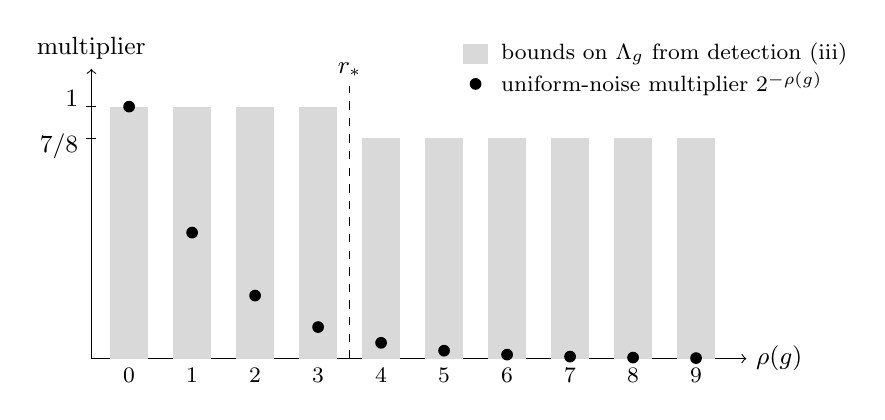
\begin{tikzpicture}[font=\small,xscale=0.8,yscale=3.2]
\draw[->] (-0.6,0) -- (9.8,0) node[right] {$\rho(\boldsymbol g)$};
\draw[->] (-0.6,0) -- (-0.6,1.15) node[above] {multiplier};
\foreach \r in {0,...,3} { \fill[gray!30] (\r-0.3,0) rectangle (\r+0.3,1); }
\foreach \r in {4,...,9} { \fill[gray!30] (\r-0.3,0) rectangle (\r+0.3,0.875); }
\foreach \r in {0,...,9} {
  \pgfmathsetmacro{\y}{2^(-\r)}
  \node[circle,fill,inner sep=1.5pt] at (\r,\y) {};
  \node[below,font=\footnotesize] at (\r,0) {$\r$};
}
\draw (-0.68,1) -- (-0.52,1) node[left,xshift=-3pt,yshift=3pt] {$1$};
\draw (-0.68,0.875) -- (-0.52,0.875) node[left,xshift=-3pt,yshift=-3pt] {$7/8$};
\draw[dashed] (3.5,0) -- (3.5,1.08) node[above] {$r_*$};
\fill[gray!30] (5.3,1.17) rectangle (5.7,1.25);
\node[right,font=\footnotesize] at (5.75,1.21) {bounds on $\Lambda_{\boldsymbol g}$ from detection (iii)};
\node[circle,fill,inner sep=1.5pt] at (5.5,1.09) {};
\node[right,font=\footnotesize] at (5.75,1.09) {uniform-noise multiplier $2^{-\rho(\boldsymbol g)}$};
\end{tikzpicture}
\caption{Multipliers against $\rho(\boldsymbol g)$, with $r_*=4$ for illustration. Bars: the bounds on $\Lambda_{\boldsymbol g}$, which $\rho(\boldsymbol g)$ does not determine. Dots: $2^{-\rho(\boldsymbol g)}$.}\label{fig:multipliers}
\end{figure}

\emph{Why only constant soundness.} The comparison needs high acceptance. If $F$ passes the latent test with probability $q$, the same computation gives $w\ge8q-7$, which is positive only when $q>7/8$. So this comparison cannot give soundness $\varepsilon$ the way Lemma~\ref{lem:foldcompare} did. It shows only that, on unsatisfiable formulas, no labeling passes the latent test with probability at least $q$, for a fixed $q>7/8$. OpenAI takes $q=0.99$.

\emph{Steps 2--5 with the extra component.} Tables now have the component $T$, so the advice experiment also gives $T_O$ and $T_O\bar\pi$ to the two provers. The $O$-prover receives $(A,T_O,AM_O)$ and the $U$-prover $(A,T_O\bar\pi,AM_O\bar\pi)$ \cite[Definition~5.2]{OAI}. Good triples, certificates, and transferred slices are defined for the functions $M\mapsto F_U(M,T)$. Lemmas~\ref{lem:goodadvice}--\ref{lem:transfer} hold with $(U,T)$ in place of $U$, with latent acceptance at least $0.99$ in place of $\val_\lambda(G_{2:2})\ge\varepsilon$, and with constants recomputed from the comparison \cite[Lemmas~5.5--5.7]{OAI}. The provers' strategies of Chapter~\ref{ch:twotwo} are unchanged \cite[Proposition~5.3]{OAI}. An entry is clean when the columns of both $T_O$ and $AM_O$ at its variable vanish, which has probability at least $\beta2^{-\dim\cW-r_{\mathrm s}}$, so Lemma~\ref{lem:clean} holds with $2^{-\dim\cW-r_{\mathrm s}}$ in place of $2^{-r_{\mathrm s}}$ \cite[Lemma~6.2]{OAI}. In the NO case and for large $k$, the decoded strategies and the repetition bound contradict each other, so no labeling passes the latent test with probability above $0.99$. With the completeness computed above, this gives OpenAI's fixed gap.

\begin{proposition}[{\cite[Proposition~6.3]{OAI}}]\label{prop:latentgap}
Fix $p_*>0$, and choose the latent gadget and the parameters of Theorem~\ref{thm:inverse} in the order of \cite[Equation~(5.4)]{OAI}. For every sufficiently large cube $k$, OpenAI's folded game $\mathcal G$, built from a parity system $\Theta$ with three distinct variables in each equation, satisfies
\[
\OPT(\Theta)\ge1-\xi\ \Longrightarrow\ \val(\mathcal G)\ge1-k\xi-p_*/2,\qquad\OPT(\Theta)\le4/5\ \Longrightarrow\ \val(\mathcal G)\le0.99.
\]
The threshold on $k$ does not depend on $\Theta$ or $\xi$.
\end{proposition}

\chapterquestions
\begin{question}\label{q:mu}
Show that $\Lambda_{\boldsymbol g}=2^{-\rho(\boldsymbol g)}$ when $a$ is uniform in $K$, which is the multiplier of the ordinary test.
\end{question}

\begin{question}\label{q:point8}
Suppose some labeling passes the latent test with probability $0.8$. What does the comparison give, and why?
\end{question}

\chapter{A fixed gap suffices}\label{ch:games}

OpenAI's folded game has soundness $0.99$ (Proposition~\ref{prop:latentgap}), far from the $\delta$ of the conjecture. Which weaker statement already implies the conjecture? Proposition~\ref{prop:fixedgap} gives one: a single fixed soundness $1-\Delta$, with completeness arbitrarily close to $1$ (Figure~\ref{fig:plane}).

\begin{proposition}\label{prop:fixedgap}
Let $\Delta\in(0,1)$. Suppose that for every $\varepsilon'\in(0,\Delta)$ there is $\ell(\varepsilon')$ such that $\GapUG_{\F_2^{\ell(\varepsilon')}}(1-\varepsilon',1-\Delta)$ is NP-hard on weighted bipartite translation games. Then for all $\varepsilon,\delta\in(0,1/2)$ there is $N$ such that $\GapUG_{\F_2^N}(1-\varepsilon,\delta)$ is NP-hard on weighted bipartite translation games.
\end{proposition}

\begin{figure}[ht]
\centering
\begin{tikzpicture}[scale=0.9,font=\small]
\fill[gray!18] (0,0) -- (6,6) -- (0,6) -- cycle;
\node[gray!60!black,align=center] at (1.6,4.4) {no gap\\$(c\le s)$};
\draw[->] (0,0) -- (6.5,0) node[below right] {completeness $c$};
\draw[->] (0,0) -- (0,6.5) node[left] {soundness $s$};
\draw[gray,dashed] (6,0) -- (6,6) -- (0,6);
\node[below] at (0,0) {$0$};
\node[below] at (3,0) {$\tfrac12$};
\draw (3,-0.08) -- (3,0.08);
\node[below] at (6,0) {$1$};
\node[left] at (0,6) {$1$};
\fill (2.8,0.3) circle (2.2pt);
\node[above,align=center] at (2.8,0.45) {Corollary~\ref{cor:half}:\\$\bigl(\tfrac{1-\varepsilon}{2},\,\delta\bigr)$};
\fill[newc] (5.9,4.8) circle (2.2pt);
\node[newc,right,align=left] at (6.15,4.8) {hypothesis of Proposition~\ref{prop:fixedgap}:\\$(1-\varepsilon',\,1-\Delta)$ for every $\varepsilon'$};
\fill[newc] (5.7,0.3) circle (2.2pt);
\node[newc,right,align=left] at (6.15,0.3) {Theorem~\ref{thm:ugt}: $(1-\varepsilon,\,\delta)$};
\draw[-{Stealth[length=2.2mm]},thick] (5.88,4.65) -- (5.72,0.48);
\node[right,align=left] at (6.15,2.6) {$n$-fold repetition\\(Proposition~\ref{prop:fixedgap})};
\end{tikzpicture}
\caption{NP-hard gap problems $(c,s)$ (schematic): the form of the conjecture, the earlier result, and the route of Proposition~\ref{prop:fixedgap}.}\label{fig:plane}
\end{figure}

\emph{The idea: repeat the game.} Heuristically, requiring $n$ independent copies of a game $H$ to be satisfied at once should give value about $\val(H)^n$. This is at least $1-n\varepsilon'$ when $\val(H)\ge1-\varepsilon'$, and exponentially small when $\val(H)\le1-\Delta$. The completeness half is a union bound, and the soundness half is Theorem~\ref{thm:rep}.

\begin{proof}[Proof of Proposition~\ref{prop:fixedgap}]
Given $\varepsilon$ and $\delta$, choose $n$ with $(1-\Delta^2/16)^n\le\delta$ and $\varepsilon/n<\Delta$, and set $\varepsilon'=\varepsilon/n$. We reduce the hypothesized hard problem to the target problem by mapping each instance $H$ of $\GapUG_{\F_2^{\ell(\varepsilon')}}(1-\varepsilon',1-\Delta)$ to $H^{\otimes n}$. Its constraints are products of translations, so it is a translation game over $\F_2^N$ with $N=n\,\ell(\varepsilon')$. Because $n$ is fixed, $H^{\otimes n}$ has size polynomial in that of $H$. It remains to check completeness and soundness.

\emph{Completeness.} Suppose $\val_\lambda(H)\ge1-\varepsilon'$, and label $H^{\otimes n}$ by $\lambda^{\otimes n}(v_1,\dots,v_n)=(\lambda(v_1),\dots,\lambda(v_n))$. This labeling fails an edge $(e_1,\dots,e_n)$ only if $\lambda$ fails some $e_i$. Each $e_i$ has law $p$, so $\lambda$ fails it with probability at most $\varepsilon'$. By a union bound, $\val(H^{\otimes n})\ge1-n\varepsilon'=1-\varepsilon$.

\emph{Soundness.} If $\val(H)\le1-\Delta$, then $\val(H^{\otimes n})\le(1-\Delta^2/16)^n\le\delta$ by Theorem~\ref{thm:rep}.
\end{proof}

\emph{Why Theorem~\ref{thm:rep} is stated for projection games.} The proof above uses projections only through Theorem~\ref{thm:rep}, and uses that theorem through one property: the bound does not depend on the alphabet. This property is needed because the proof chooses $n$ first, then $\varepsilon'=\varepsilon/n$, and only then the alphabet $\F_2^{\ell(\varepsilon')}$. In games whose edges carry arbitrary relations instead of maps (general two-prover games), Holenstein's repetition bound is $\bigl(1-\Delta^3/6000\bigr)^{n/\log(|\Sigma||\Sigma'|)}$ for alphabets $\Sigma$ and $\Sigma'$ \cite[Theorem~2.5]{Hol09}, which weakens as the alphabets grow. Some dependence on the alphabet is necessary. Feige and Verbitsky give games of value at most $3/4$ for which the number of repetitions needed to bring the value below $1/8$ grows without bound with the number of labels \cite{FV02}, \cite[Section~1]{Hol09}. With a bound that weakens as the alphabet grows, $n$ would have to grow with $\ell(\varepsilon/n)$, which itself depends on $n$ (Question~\ref{q:holenstein}).
\paragraph{Loops and weights.} OpenAI's folded game is a weighted translation game, and its random edge can be a loop, for example when $a=0$ or $l=0$. So the folded game is not yet a game in the sense of Definition~\ref{def:ug}. Part~I could delete loops and copy edges because 2-to-2 games may have parallel edges, while Theorem~\ref{thm:ugt} needs simple bipartite graphs. OpenAI's Lemma~7.1 turns this weighted game with loops into an unweighted simple bipartite translation game. The lemma \emph{rounds} each weight to an integer multiple of a common unit, replaces each edge by as many copies as its rounded weight has units, and then \emph{subdivides} each copy into a path of four edges through three new vertices. Subdivision turns a game $H$ into a game of value exactly $1-(1-\val(H))/4$, and rounding changes the value by an amount that can be made arbitrarily small \cite[Lemma~7.1 and Equation~(7.2)]{OAI}. So a game with completeness $1-\varepsilon'$ and soundness $1-\Delta$ becomes one with completeness about $1-\varepsilon'/4$ and soundness about $1-\Delta/4$, with errors as small as desired.
\paragraph{Assembling Theorem~\ref{thm:ugt}.} Theorem~\ref{thm:ugt} asks, for all $\varepsilon,\delta\in(0,1/2)$, for a polynomial-time reduction from 3SAT to unweighted translation games over some $\F_2^N$ on simple bipartite graphs, with completeness $1-\varepsilon$ and soundness $\delta$. By Proposition~\ref{prop:latentgap}, OpenAI's folded game has value at least $1-k\xi-p_*/2$ on satisfiable formulas (Figure~\ref{fig:pipeline} tracks this bound through the reduction) and at most $0.99$ on unsatisfiable ones. Rounding and subdivision give an unweighted simple bipartite translation game with soundness at most $1-1/800$ \cite[Lemma~7.1]{OAI}, and with completeness $1-\varepsilon'$, where $\varepsilon'$ can be made as small as desired by the choice of $p_*$, the rounding precision $\vartheta$ of \cite[Lemma~7.1]{OAI} (called $\tau$ there), $k$, and $\xi$. Proposition~\ref{prop:fixedgap} with $\Delta=1/800$ then gives Theorem~\ref{thm:ugt}. The games from Lemma~7.1 are unweighted and simple, and so are their repetitions: the product of uniform laws on $E$ is uniform on $E^n$, and since the game is simple, distinct tuples of edges join distinct pairs of vertex tuples. The parameters are chosen in the order $(\varepsilon,\delta)\to n\to(p_*,\vartheta)\to r_*\to(\alpha,r_{\mathrm s})\to\ell\to(\cV,C,\mu)\to k\to\xi$ (simplified from \cite[Equation~(5.4)]{OAI}). The assembly in this paragraph corresponds to the last two arrows of Figure~\ref{fig:dependency}.

\begin{figure}[ht]
\centering
\begin{tikzpicture}[font=\small,
  box/.style={draw,rounded corners=2pt,align=center,inner sep=4pt,minimum height=2.2em},
  arr/.style={-{Stealth[length=2mm]}},
  lab/.style={font=\footnotesize,align=center}]
\node[box] (sat) {3SAT};
\node[box,right=1.5cm of sat] (lin) {parity equations\\$\OPT(\Theta)\ge1-\xi$};
\node[box,right=1.5cm of lin] (out) {$k$ equations, all satisfied\\by a best assignment\\with probability $\ge1-k\xi$};
\draw[arr] (sat) -- node[lab,above] {H\aa stad} node[lab,below] {Thm~\ref{thm:hastad}} (lin);
\draw[arr] (lin) -- node[lab,above] {sample $k$} node[lab,below] {equations} (out);
\node[box,below left=1.3cm and -0.4cm of out] (old) {2-to-2 test, split\\value $\le\tfrac12$};
\node[box,draw=newc,text=newc,below right=1.3cm and -0.4cm of out] (new) {latent test\\value $\ge1-k\xi-p_*/2$};
\draw[arr] (out) -- node[lab,left] {inner test\\(Ch.~\ref{ch:inner})} (old);
\draw[arr,newc,thick] (out) -- node[lab,right,text=newc] {inner test\\(Ch.~\ref{ch:openai})} (new);
\node[box,below=1.4cm of new] (fin) {Unique Games\\value $\ge1-\varepsilon$};
\draw[arr] (new) -- node[lab,right,align=left] {rounding, subdivision,\\repetition (Prop.~\ref{prop:fixedgap})} (fin);
\node[lab,below=0.35cm of old] {repetition does not increase the value};
\end{tikzpicture}
\caption{Completeness after each step in the YES case, and the upper bound $1/2$ for the 2-to-2 route. The replacement probability $\beta$ of the smooth game (Chapter~\ref{ch:outer}) matters only in the soundness proofs (Chapters~\ref{ch:twotwo} and~\ref{ch:openai}).}\label{fig:pipeline}
\end{figure}

\paragraph{Part~I and Part~II side by side.} The table lists everything that changes between the two proofs.
\begin{center}\small
\begin{tabular}{@{}p{2.1cm}p{5.6cm}p{7.4cm}@{}}
 & Part~I (Theorem~\ref{thm:2to2}) & Part~II (Theorem~\ref{thm:ugt})\\\hline
tables & $M\in\Hom(L_U,K)$ & $P=(M,T)\in\Hom(L_U,\cV)$, $\cV=K\oplus\cW$\\
encoding & $M\mapsto Mz$ & $P\mapsto C(Pz)$\\
test & 2-to-2 test, $a$ uniform in $K$ & latent test, $a\sim\mu$ on $\cV$\\
constraints & 2-to-2 & translations\\
completeness & $\ge1-k\xi-\rho_0$ & $\ge1-k\xi-p_*/2$\\
Step 1 & folding (Lemma~\ref{lem:foldcompare}) & Fourier comparison, which needs acceptance above $7/8$\\
Steps 2--5 & Chapter~\ref{ch:twotwo} & with $(U,T)$ in place of $U$, and $2^{-\dim\cW-r_{\mathrm s}}$ in Lemma~\ref{lem:clean}\\
soundness & $\varepsilon$ & $0.99$, then \cite[Lemma~7.1]{OAI} and Proposition~\ref{prop:fixedgap}\\
loops, weights & loops deleted, edges copied (parallel edges allowed) & rounding and subdivision\\
\end{tabular}
\end{center}

\chapternotes
OpenAI's overview \cite[Section~1.4]{OAI} presents the latent gadget (Lemma~\ref{lem:latent}) and the Fourier comparison as new, and the other ingredients as adapted from earlier work (Notes to Chapter~\ref{ch:twotwo}).

\chapterquestions
\begin{question}\label{q:holenstein}
Suppose the repetition bound for alphabet $\F_2^\ell$ were $\zeta^{n/\ell}$, with $0<\zeta<1$ depending only on $\Delta$ (the form of Holenstein's bound). For which growth rates of $\ell(\varepsilon')$ does the proof of Proposition~\ref{prop:fixedgap} still work?
\end{question}

\begin{question}\label{q:subdivision}
Let $H$ be a weighted translation game. Replace each edge $e=(v,w)$, with offset $b_e$, by a path $v,x_1,x_2,x_3,w$ through three new vertices, and give the four edges of the path offsets with sum $b_e$ and weight $p_e/4$ each. Show that the new game has value exactly $1-(1-\val(H))/4$.
\end{question}


\appendix
\chapter{Answers to the questions}\label{app:answers}

\paragraph{Question~\ref{q:oddcycle}.} $\val(G)=1-1/L$. A labeling that satisfies every edge has $\lambda(v_{i+1})=\lambda(v_i)+1$ for all $i$, and summing around the cycle gives $\lambda(v_1)=\lambda(v_1)+L=\lambda(v_1)+1$, as in Figure~\ref{fig:ugexample}. So every labeling fails at least one of the $L$ equally weighted edges, and $\val(G)\le1-1/L$. The labeling $\lambda(v_i)=i\bmod2$ satisfies the edges $(v_i,v_{i+1})$ for $i<L$, so $\val(G)\ge1-1/L$.

\paragraph{Question~\ref{q:propagation}.} In a connected component, fix a spanning tree and a label at its root. A permutation constraint on a tree edge leaves exactly one label at the far endpoint that satisfies the edge. So each of the $|K|$ root labels determines one labeling of the component, and checking each such labeling on every edge takes polynomial time. A 2-to-2 constraint relates each label at one endpoint to two labels at the other. Each root label then leaves two choices at every tree edge, so the number of labelings that satisfy the tree edges is exponential in the number of tree edges, and enumerating these labelings takes exponential time.

\paragraph{Question~\ref{q:evvexact}.} By Lemma~\ref{lem:evv}, it suffices to find a labeling with value $1-\bigl(1-\OPT(\Theta)\bigr)/3$. Take an assignment $\mathbf x$ that attains $\OPT(\Theta)$, and label each variable by its value. Label each equation $\theta$ by the restriction of $\mathbf x$ to the variables of $\theta$ if $\mathbf x$ satisfies $\theta$, and otherwise by that restriction with one variable flipped, so that the label satisfies $\theta$. Given $\theta$, the random edge then fails with probability $0$ in the first case, and with probability exactly $1/3$ in the second, since the label differs from $\mathbf x$ at exactly one of the three variables. So this labeling has value $1-\tfrac13\Prob_{\theta\sim p}[\mathbf x\text{ violates }\theta]=1-\bigl(1-\OPT(\Theta)\bigr)/3$.

\paragraph{Question~\ref{q:pibar}.} With coordinates $(z_0,x_3)$ on $L_O$, restriction to $x_3$ is $z\mapsto(z_0,\,bz_0+\phi_1+\phi_2)$, with matrix $\begin{pmatrix}1&0&0\\ b&1&1\end{pmatrix}$. With coordinates $(z_0,x_1)$, restriction to $x_1$ is $z\mapsto(z_0,\phi_1)$, with matrix $\begin{pmatrix}1&0&0\\0&1&0\end{pmatrix}$. Both keep the homogeneous coordinate. On the bits alone, restriction to $x_1$ is the linear map $(\phi_1,\phi_2)\mapsto\phi_1$, while restriction to $x_3$ is $(\phi_1,\phi_2)\mapsto b+\phi_1+\phi_2$, which is linear only when $b=0$.

\paragraph{Question~\ref{q:homog}.} Every label $z$ has $z_0=1$, so every encoding satisfies $f_z(M^{+h})=Mz+hz_0=f_z(M)+h$. Folding imposes this identity, which all encodings share, on every labeling. Adding $h$ to the column at a coordinate $i\ne0$ gives $f_z(M+he_i^\top)=f_z(M)+hz_i$, and the change $hz_i$ depends on the label. So this shift changes different encodings by different amounts, and folding cannot impose it.

\paragraph{Question~\ref{q:disagree}.} The probability is $2^{-\ell}$. Since $(P'\bar\pi_i)z_i=P'(\bar\pi_iz_i)$, the two values are $P'(\bar\pi_1z_1)$ and $P'(\bar\pi_2z_2)$, and they agree exactly when $P'(\bar\pi_1z_1-\bar\pi_2z_2)=0$. Since $\bar\pi_1z_1-\bar\pi_2z_2\ne0$ and $P'$ is a uniform linear map $L_O\to K$, this vector $P'(\bar\pi_1z_1-\bar\pi_2z_2)$ is uniform on $K$. So encodings of labels with different restrictions disagree on a $1-2^{-\ell}$ fraction of the tables on $O$.

\paragraph{Question~\ref{q:rowslices}.} Fix $d\in\F_2^\ell\setminus\{0\}$, write $t'=M^\top d$, and let $f(M)=Mt'$. On the row slice $M^\top d=t'$, the function $f$ is the encoding $f_{t'}$.

\emph{$f$ passes the equality test with probability at least $1/4$.} If $a^\top d=0$ and $l^\top t'=0$, then $(M+al^\top)^\top d=M^\top d=t'$, so the step stays in its row slice, and $f(M+al^\top)=Mt'+a(l^\top t')=f(M)$. Given $M$, the two events are independent, with probabilities $1/2$ and at least $1/2$.

\emph{$f$ agrees with every target on a small fraction of every slice cut out by column equations alone.} Fix such a slice, $Mq_j=t_j$ for $j=1,\dots,r$, and a target $Mz+u$. On the slice, $t'$ is uniform on a coset of the space $\{y\in\F_2^m:y^\top q_j=0\text{ for all }j\}$, whose dimension is at least $m-r$. The event $f(M)=Mz+u$ reads $M(t'-z)=u$. The vector $t'-z$ lies in $\Span\{q_j\}$ with probability at most $2^r\cdot2^{-(m-r)}$. Otherwise, given $t'$, the vector $M(t'-z)$ is uniform on a coset of the hyperplane $\{y\in K:d^\top y=0\}$, so $M(t'-z)=u$ has probability at most $2^{1-\ell}$. Hence the agreement on the slice is at most $2^{1-\ell}+2^{2r-m}$.

The function of Example~\ref{ex:zoomout} has small agreement on every slice cut out by row equations alone. Write the row equations as $AM=S$, with $s=\rank A\le r$, and fix a target $Mz+u$ with $z=z'+\nu q$ as in Example~\ref{ex:zoomout}. Given the nonempty row fiber, $t=Mq$ is uniform on a coset of $\ker A$, which has $2^{\ell-s}$ elements. At most one $t$ has $z_t=z'$, and that $t$ contributes at most $2^{-(\ell-s)}$. For the other $t$, the vector $z_t-z'$ is independent of $q$, so given $Mq=t$ the vector $M(z_t-z')$ is uniform on a coset of $\ker A$ and equals $\nu t+u$ with probability at most $2^{-(\ell-s)}$. So the agreement is at most $2^{1+r-\ell}$. So a theorem of the form of Theorem~\ref{thm:inverse} must allow both row and column equations.

\paragraph{Question~\ref{q:beta}.} \emph{$\beta=1$.} Every entry is replaced. Given $U$ and the positions of the replacing variables, the pullbacks $M_O\bar\pi$ form a subspace of $\Hom(L_U,K)$ of dimension $\ell(1+k)$, because $\bar\pi$ is onto and $L_O$ has dimension $1+k$. There are $3^k$ choices of positions, so the law of $M_O\bar\pi$ is supported on at most $3^k2^{\ell(1+k)}$ of the $2^{\ell(1+2k)}$ tables. Its total variation distance from the uniform law is therefore at least $1-(3\cdot2^{-\ell})^k$. So the conclusion of Lemma~\ref{lem:tv} fails, and the proof of Lemma~\ref{lem:transfer}, which carries good advice from uniform tables to pullbacks, no longer applies. Steps~1, 2, and~5 still hold, and so does Lemma~\ref{lem:goodadvice}, which concerns uniform tables. Step~4 fails.

\emph{$\beta=1/k$.} Now $k\beta^2=1/k\to0$, so Lemma~\ref{lem:tv} holds, but Step~5 fails. With probability $(1-1/k)^k\ge1/4$ for $k\ge2$, no entry is replaced. Then $O=U$, the map $\bar\pi$ is the identity, both provers receive the same input, and two copies of one deterministic strategy succeed. So no bound that tends to $0$ as $k$ grows can hold. Correspondingly, the bound of Lemma~\ref{lem:clean} becomes $\bigl(1-2^{-r_{\mathrm s}}/(3600k)\bigr)^k$, which tends to $\exp(-2^{-r_{\mathrm s}}/3600)$.

\paragraph{Question~\ref{q:erasure}.} A constant would create agreement instead of erasing it. A function $f'$ that took a constant value $y$ on $\mathcal B$ would agree with the target $M\mapsto M0+y$ at every table of $\mathcal B$. Every slice inside the row fiber of a good triple would then carry agreement $1$, and Theorem~\ref{thm:inverse} would not be contradicted. Each new value equals a fixed target with probability exactly $2^{-\ell}$, so the expected agreement of the new values with a target on a slice is at most $2^{-\ell}<\alpha/8$. Hoeffding's inequality, with a union bound over the at most $2^{(2r_{\mathrm s}+1)(\ell+m)}$ descriptions of slices and targets, keeps the contribution of the resampled values below $\alpha/4$ on every slice, for every target.

\paragraph{Question~\ref{q:mu}.} For $a\in K$, the conditions $g_i(a)=0$ for all $i$ say that $a$ lies in the kernel of the linear map $K\to\F_2^m$, $a\mapsto(g_0(a),\dots,g_{m-1}(a))$. The rank of this map is $\dim\Span\{g_i|_K\}=\rho(\boldsymbol g)$, so its kernel has dimension $\ell-\rho(\boldsymbol g)$. A uniform $a\in K$ lies in it with probability $2^{\ell-\rho(\boldsymbol g)}/2^\ell=2^{-\rho(\boldsymbol g)}$.

\paragraph{Question~\ref{q:point8}.} Nothing useful. With $q=0.8$ the computation gives $w\ge8q-7=-0.6$, which is no bound. The trivial character contributes $2^{-\ell}$ to $w$, and $2^{-\ell}\to0$ as $\ell$ grows. So the comparison does not give the acceptance bound independent of $\ell$ that Theorem~\ref{thm:inverse} needs.

\paragraph{Question~\ref{q:holenstein}.} The proof needs $n$ with $\varepsilon/n<\Delta$ and $\zeta^{n/\ell(\varepsilon/n)}\le\delta$, that is,
\[
\frac{n}{\ell(\varepsilon/n)}\ \ge\ \frac{\log(1/\delta)}{\log(1/\zeta)}.
\]
With $\varepsilon'=\varepsilon/n$, the left side is $n/\ell(\varepsilon')=\varepsilon/\bigl(\varepsilon'\ell(\varepsilon')\bigr)$. So such $n$ exists for every $\delta$ exactly when $\varepsilon'\ell(\varepsilon')$ has infimum $0$ along $\varepsilon'=\varepsilon/n$. The infimum is $0$ when $\ell(\varepsilon')=O(\log(1/\varepsilon'))$ or $\ell(\varepsilon')=O(\varepsilon'^{-1/2})$, and positive when $\varepsilon'\ell(\varepsilon')$ is bounded below by a positive constant.

\paragraph{Question~\ref{q:subdivision}.} Let $\lambda'$ label the new game, and let $\lambda$ be the restriction of $\lambda'$ to the vertices of $H$. The four translations of a path compose to the translation of $e$, so if $\lambda$ fails $e$, then $\lambda'$ fails at least one of the four path edges. Hence $\val_{\lambda'}\le1-\tfrac14\Prob_{e\sim p}[\lambda\text{ fails }e]\le1-(1-\val(H))/4$. Conversely, take a labeling $\lambda$ of $H$ with $\val_\lambda(H)=\val(H)$, and on each path choose the labels of $x_1$, $x_2$, and $x_3$ so that the first three path edges are satisfied. The fourth edge is then satisfied exactly when $\lambda$ satisfies $e$, so the extended labeling has value $1-(1-\val(H))/4$.

\chapter{Notation}\label{app:notation}

{\small
\renewcommand{\arraystretch}{1.15}
\begin{longtable}{@{}p{3.4cm}p{10.4cm}r@{}}
symbol & meaning & page\\\hline
\endhead
$K$ & alphabet of a unique game; from Chapter~\ref{ch:inner} on, $K=\F_2^\ell$ & \pageref{def:ug}\\
$p$ & distribution on the edges of a game (its weights); for a parity system, on its equations & \pageref{def:ug}\\
$\val_\lambda(G)$, $\val(G)$ & value of a labeling $\lambda$ of a game $G$, and the maximum value over labelings & \pageref{def:ug}\\
$\GapUG_K(c,s)$ & given a unique game over $K$ with $\val\ge c$ or $\val\le s$, deciding which holds & \pageref{nt:gap}\\
$\Theta$, $\OPT(\Theta)$, $\xi$ & parity system, its optimum, H\aa stad's parameter & \pageref{thm:hastad}\\
$G_\Theta$ & equation-versus-variable game & \pageref{def:evv}\\
$G^{\otimes n}$ & $n$-fold repetition of a projection game & \pageref{def:rep}\\
$k$, $\beta$, $(U,O)$ & number of equations in $U$, replacement probability, random edge of the smooth game & \pageref{def:smooth}\\
$L_Q$, $z_0$, $\bar\pi$ & space of a vertex $Q$ (the labels of $Q$ are the vectors of $L_Q$ with $z_0=1$); homogeneous coordinate; linear restriction $L_U\to L_O$ & \pageref{nt:labels}\\
$m$ & $\dim L_U=1+2k$ & \pageref{nt:labels}\\
$\ell$ & $K=\F_2^\ell$ in the constructed games & \pageref{nt:clouds}\\
$P$, $M$, $\Mat_{\ell,m}$ & table on a vertex; table on a first endpoint, an element of $\Mat_{\ell,m}=\Hom(L_U,K)$ (in Part~II, the $K$-component of $P$) & \pageref{nt:clouds}\\
$f_z$ & encoding of a label $z$ & \pageref{nt:clouds}\\
$P'\bar\pi$ & pullback of a table $P'$ on $O$ & \pageref{nt:shared}\\
$a$, $l$ & random vectors of the tests & \pageref{def:shortcode}\\
$P^{+h}$, $e_0$, $F_Q$ & $P+he_0^\top$, the basis vector of the homogeneous coordinate, restored function & \pageref{nt:folding}\\
$G_{2:2}$, $\rho_0$ & the 2-to-2 game, the total probability of its loops & \pageref{def:G22}\\
$\eta$, $\alpha$, $r_{\mathrm s}$ & parameters of the inverse theorem & \pageref{thm:inverse}\\
$A$, $M_O$, $S_O$ & advice experiment: row combinations, hidden table, advice $AM_O$ & \pageref{def:advice}\\
good triple, certificate & a triple $(U,A,S)$ such that, for some at most $r_{\mathrm s}$ column equations $Mq_j=t_j$, the slice $\{M:AM=S,\ Mq_j=t_j\}$ is nonempty and $F_U$ agrees with some $Mz+u$ on at least an $\alpha/2$ fraction of the slice; those equations and that target & \pageref{nt:good}\\
$Z$, $\mathcal A$ & span of the certificate's column vectors, the set of candidate labels & \pageref{lem:labelset}\\
$v_k$ & total variation bound for pullbacks & \pageref{lem:tv}\\
$D$, $z'$, $\mathcal S'$ & data that determine both inputs, restricted target vector, transferred slice & \pageref{nt:transfer}\\
$\gamma_1$, $\gamma$ & lower bound on the probability that $D$ has the properties of Lemma~\ref{lem:transfer}; lower bound on the success of the decoded strategies & \pageref{lem:transfer}, \pageref{prop:decoding}\\
clean entry, $p_A$ & replaced entry whose advice column is zero (in Part~II, also the column of $T_O$), the probability of this event & \pageref{nt:clean}\\
$\cV$, $C$, $\mu$ & latent gadget: space containing $K$, nonlinear encoding map $\cV\to K$, latent noise & \pageref{lem:latent}\\
$p_*$, $r_*$ & bound in property (ii); rank from which property (iii) guarantees detection & \pageref{lem:latent}\\
$\Lambda_{\boldsymbol g}$, $\rho(\boldsymbol g)$, $\tau$ & multiplier of a character, $\rho(\boldsymbol g)=\dim\Span\{g_i|_K\}$, ordinary-test bound & \pageref{nt:comparison}\\
$\cW$, $T$ & complement of $K$ in $\cV$, extra component of a table & \pageref{nt:comparison}\\
$\Delta$, $n$ & the hypothesized soundness is $1-\Delta$; number of repetitions & \pageref{prop:fixedgap}\\
\end{longtable}
}


\backmatter
\begin{thebibliography}{99}
\bibitem{OAI} OpenAI, \emph{The Unique Games Theorem}, preprint, September 23, 2026. \url{https://github.com/openai/math}
\bibitem{Khot10} S.~Khot, On the Unique Games Conjecture, survey, CCC 2010.
\bibitem{DKKMS} I.~Dinur, S.~Khot, G.~Kindler, D.~Minzer, and M.~Safra, Towards a proof of the 2-to-1 games conjecture?, Theory Comput.\ 21 (2025), no.~11, 1--50. Conference version STOC 2018.
\bibitem{KMS17} S.~Khot, D.~Minzer, and M.~Safra, On independent sets, 2-to-2 games, and Grassmann graphs, Theory Comput.\ 21 (2025), no.~10, 1--55. Conference version STOC 2017.
\bibitem{Ver26} R.~Vershynin, \emph{High-Dimensional Probability}, 2nd ed., version of May 28, 2026.
\bibitem{DKKMS21} I.~Dinur, S.~Khot, G.~Kindler, D.~Minzer, and M.~Safra, On non-optimally expanding sets in Grassmann graphs, Israel J.\ Math.\ 243 (2021), 377--420. Conference version STOC 2018.
\bibitem{BGS98} M.~Bellare, O.~Goldreich, and M.~Sudan, Free bits, PCPs, and nonapproximability---towards tight results, SIAM J.\ Comput.\ 27 (1998), 804--915.
\bibitem{KS13} S.~Khot and M.~Safra, A two-prover one-round game with strong soundness, Theory Comput.\ 9 (2013), 863--887.
\bibitem{BKS18} B.~Barak, P.~K.~Kothari, and D.~Steurer, Small-set expansion in shortcode graph and the 2-to-2 conjecture, ITCS 2019.
\bibitem{KMS23} S.~Khot, D.~Minzer, and M.~Safra, Pseudorandom sets in Grassmann graph have near-perfect expansion, Ann.\ of Math.\ 198 (2023), 1--92. Conference version FOCS 2018.
\bibitem{Khot02} S.~Khot, On the power of unique 2-prover 1-round games, STOC 2002, 767--775.
\bibitem{Khot19} S.~Khot, \emph{On the Proof of the 2-to-2 Games Conjecture}, expository article, 2019. \url{https://cs.nyu.edu/~khot/PCP-Spring-20/2-to-2-Exposition.pdf}
\bibitem{Hastad01} J.~H\aa stad, Some optimal inapproximability results, J.\ ACM 48 (2001), 798--859. Theorem numbers follow the author's manuscript of February 18, 2002.
\bibitem{AB09} S.~Arora and B.~Barak, \emph{Computational Complexity: A Modern Approach}, Cambridge University Press, 2009.
\bibitem{Rao11} A.~Rao, Parallel repetition in projection games and a concentration bound, SIAM J.\ Comput.\ 40 (2011), 1871--1891.
\bibitem{DS14} I.~Dinur and D.~Steurer, Analytical approach to parallel repetition, STOC 2014, 624--633.
\bibitem{Hol09} T.~Holenstein, Parallel repetition: simplifications and the no-signaling case, Theory Comput.\ 5 (2009), 141--172.
\bibitem{FV02} U.~Feige and O.~Verbitsky, Error reduction by parallel repetition---a negative result, Combinatorica 22 (2002), 461--478. Conference version CCC 1996.
\end{thebibliography}

\end{document}
